\section{Implementation}
\label{sec:Implementation}

\subsection{Frontend}
There are many mature SPA frameworks today, such as Vue.js, ReactJS, Angular.js, Angular, and so on. Since the developer is familiar with Angular, the frontend part of the project is implemented using Angular, which comes with almost everything we need, from powerful templates to fast rendering, data management, HTTP services, form handling, and so much more. Moreover, Angular provides a UI component library called Angular Material,
which is inspired by Google Material Design. Angular Material components help in constructing attractive, consistent, and functional web pages and web applications while adhering to modern web design principles like browser portability, device independence, and graceful degradation. It helps in creating faster, beautiful, and responsive websites.

\subsubsection{Overview of Frontend Folder Structure}
The Angular uses the concept of Angular Modules to group the related features. This gives us a helpful starting point to organize the folder structure. Each Module should get its folder named after the Module name. The Angular does not make any distinction between the Modules. However, based on how we made use of modules, we classified our modules into such categories: guard, model, pipe, service, and component. Figure \ref{fig:Frontend Folder Structure} shows the final structure of our frontend application.

\begin{figure}[htbp]
  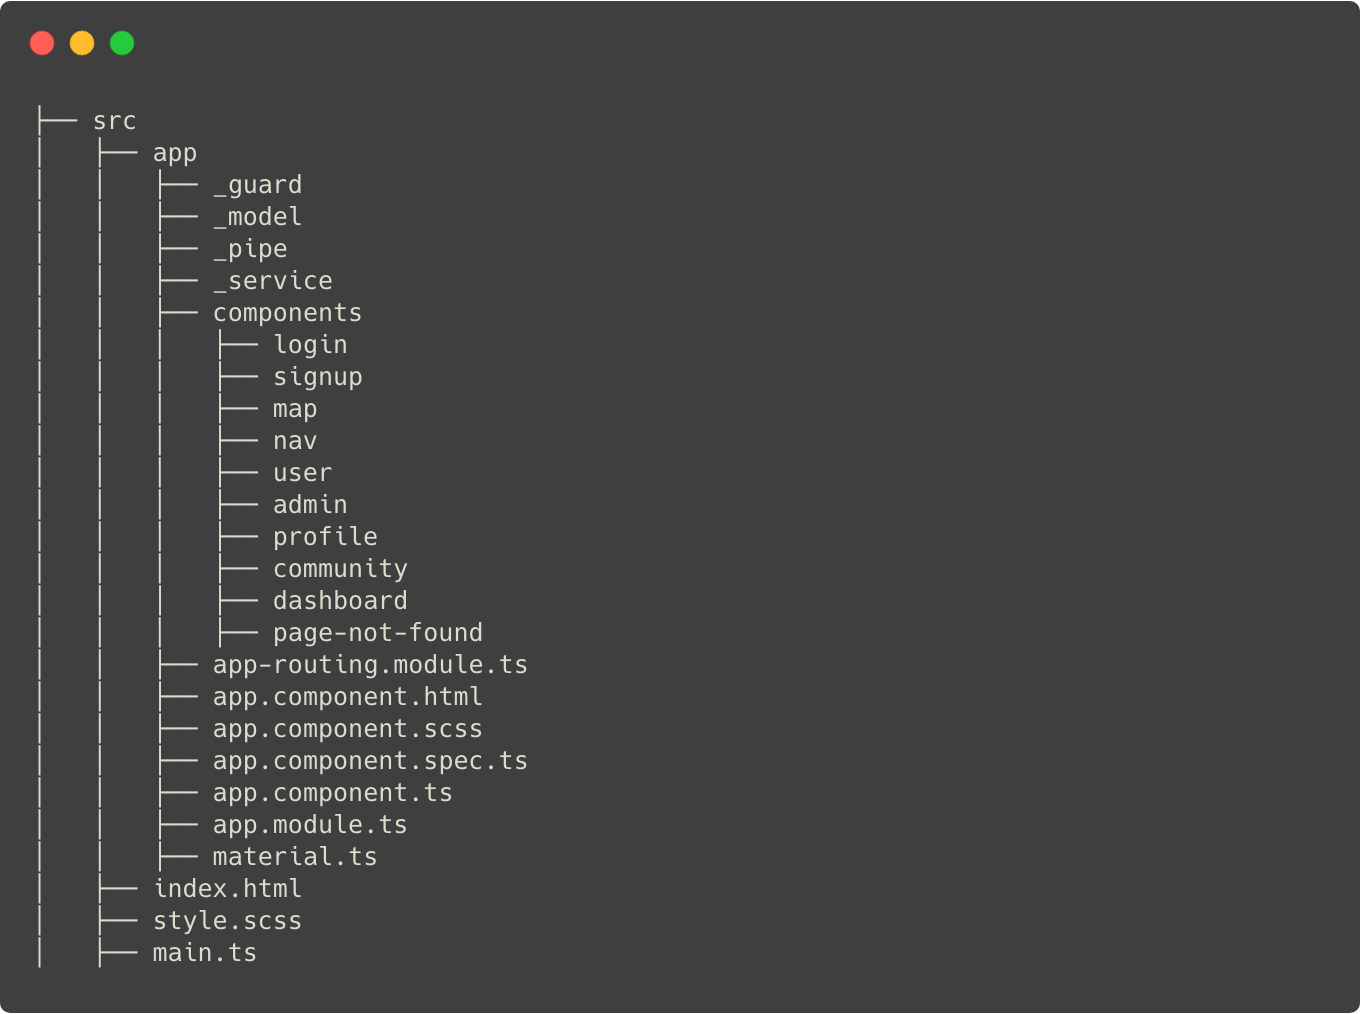
\includegraphics[width=\textwidth]{section04/assets/Frontend.png}
  \caption{Frontend Folder Structure}
  \label{fig:Frontend Folder Structure}
\end{figure}

\subsubsection{GUI Implementation}
In our design, the user must register to log in before he can use the application, so the home page is the login page. Luckily, Angular provides multiple routing guards, and the CanActivate interface is a good way for us to implement our own authentication routing. In addition, as we mentioned in Section \ref{sec:Requirements>Non-Functional Requirements} Non-Functional Requirements, every form must be validated by the client side before being submitted to the server side. The Implementation of GUI is listed below:

\begin{enumerate}
  \item The ``Sign Up'' form requires the user to enter a unique and valid email, first name, last name, password, and confirmed password. The user can click the icon on the right of the password input to make his password visible or invisible. Also, the ``clear'' button on the left bottom corner is used to clear all inputs of the ``Sign Up'' form. The user can also click the ``Log in instead'' button to be redirected to the ``Log In'' page if he already has an account. Figure \ref{fig:GUI signup} is the interface of the ``Sign Up'' page.

  \item The ``Log In'' form requires the user to enter the email and the password. Also, the user can access the ``Sign Up'' page via the ``Create account'' button on the bottom. Figure \ref{fig:GUI login} is the interface of the ``Log In'' page.

  \begin{figure}
  \centering
    \begin{subfigure}{.5\textwidth}
      \centering
      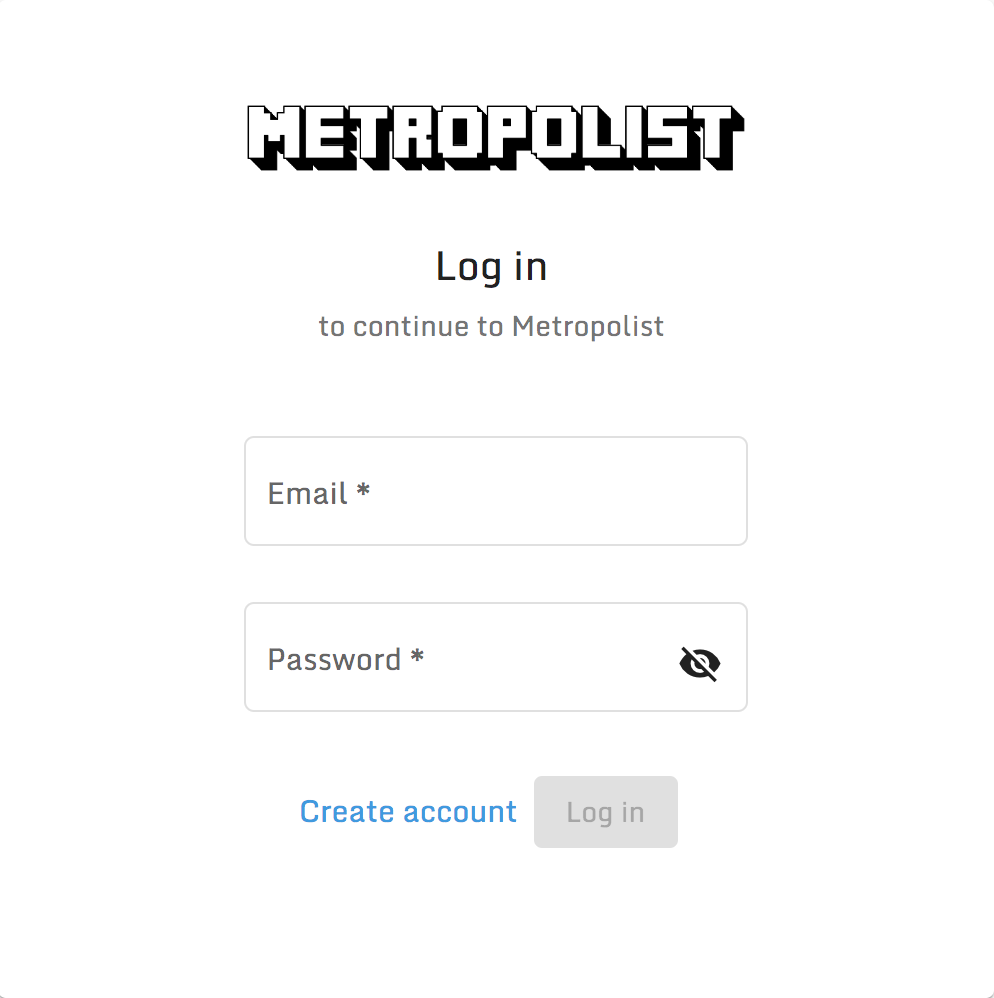
\includegraphics[width=.99\textwidth]{section04/assets/GUI-login-small.png}
      \caption{Login page}
      \label{fig:GUI login}
    \end{subfigure}%
    \begin{subfigure}{.5\textwidth}
      \centering
      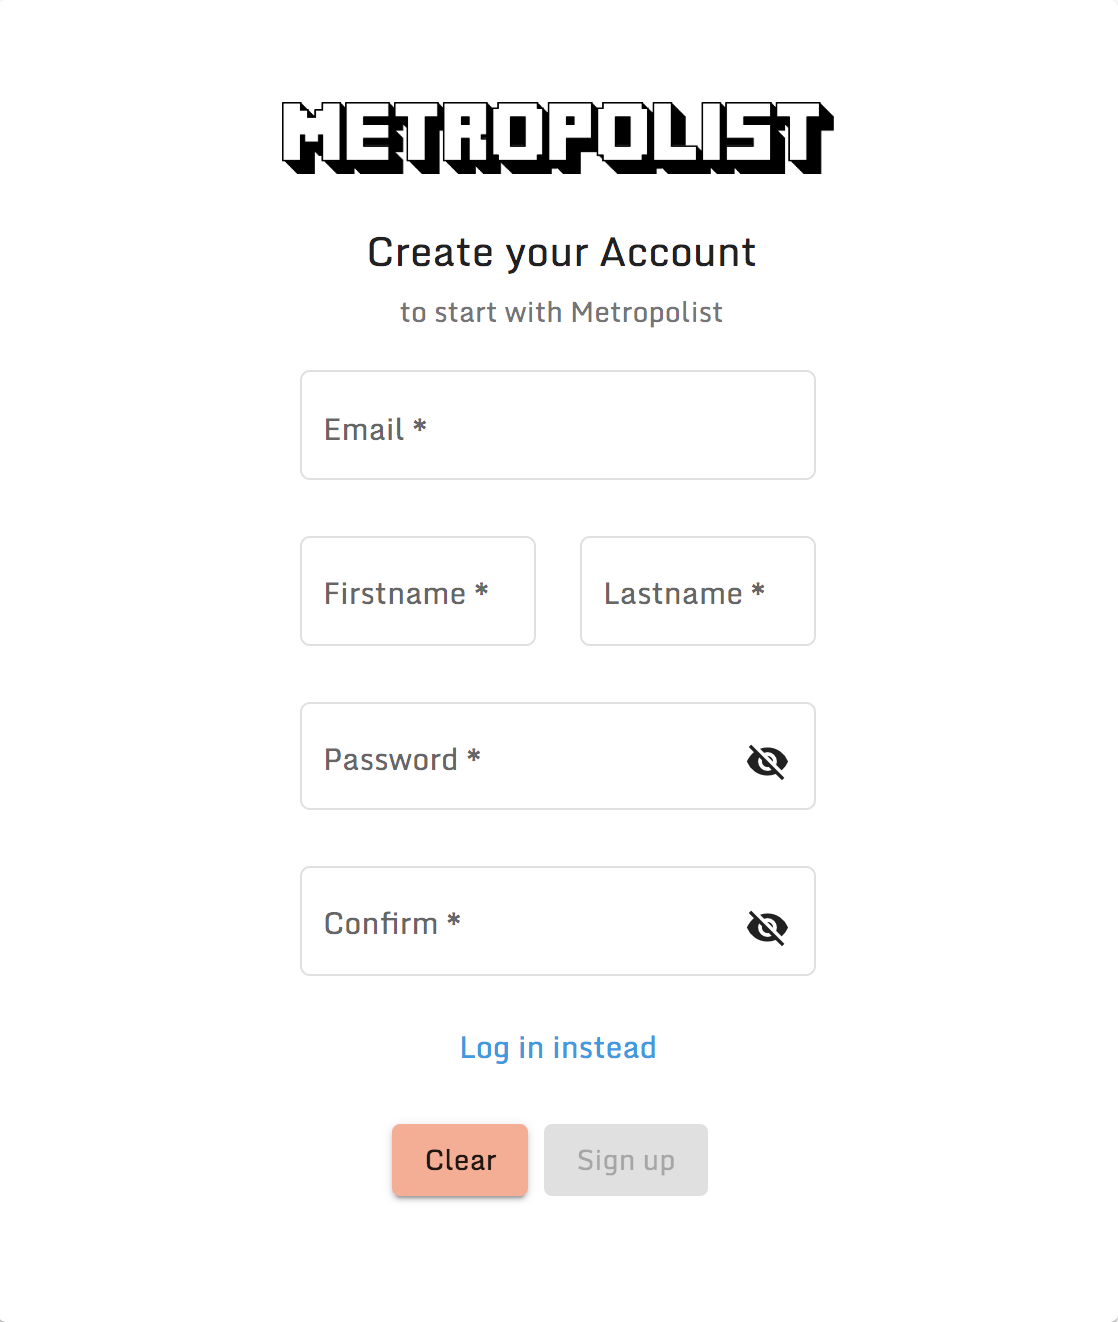
\includegraphics[width=.99\textwidth]{section04/assets/GUI-signup-small.png}
      \caption{Signup page}
      \label{fig:GUI signup}
    \end{subfigure}
    \caption{Login and Signup pages}
    \label{fig:Login and Signup pages}
  \end{figure}

  % \begin{figure}
  % \centering
  % \begin{minipage}{.5\textwidth}
  %   \centering
  %   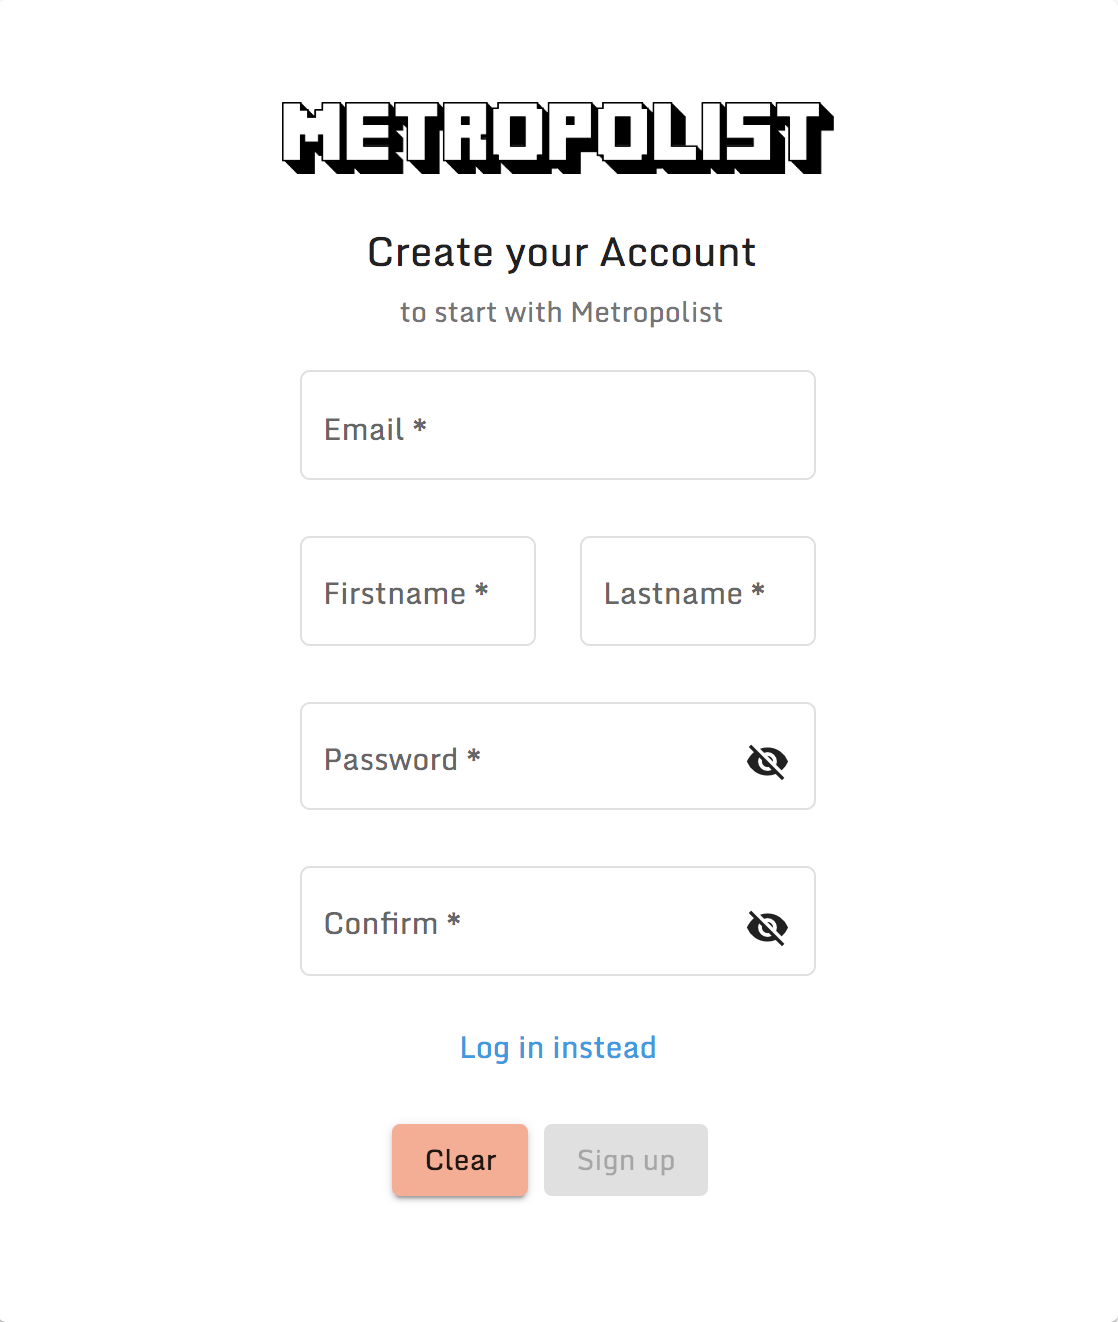
\includegraphics[width=\textwidth]{section04/assets/GUI-signup-small.png}
  %   \caption{Signup page}
  %   \label{fig:GUI signup}
  % \end{minipage}%
  % \begin{minipage}{.5\textwidth}
  %   \centering
  %   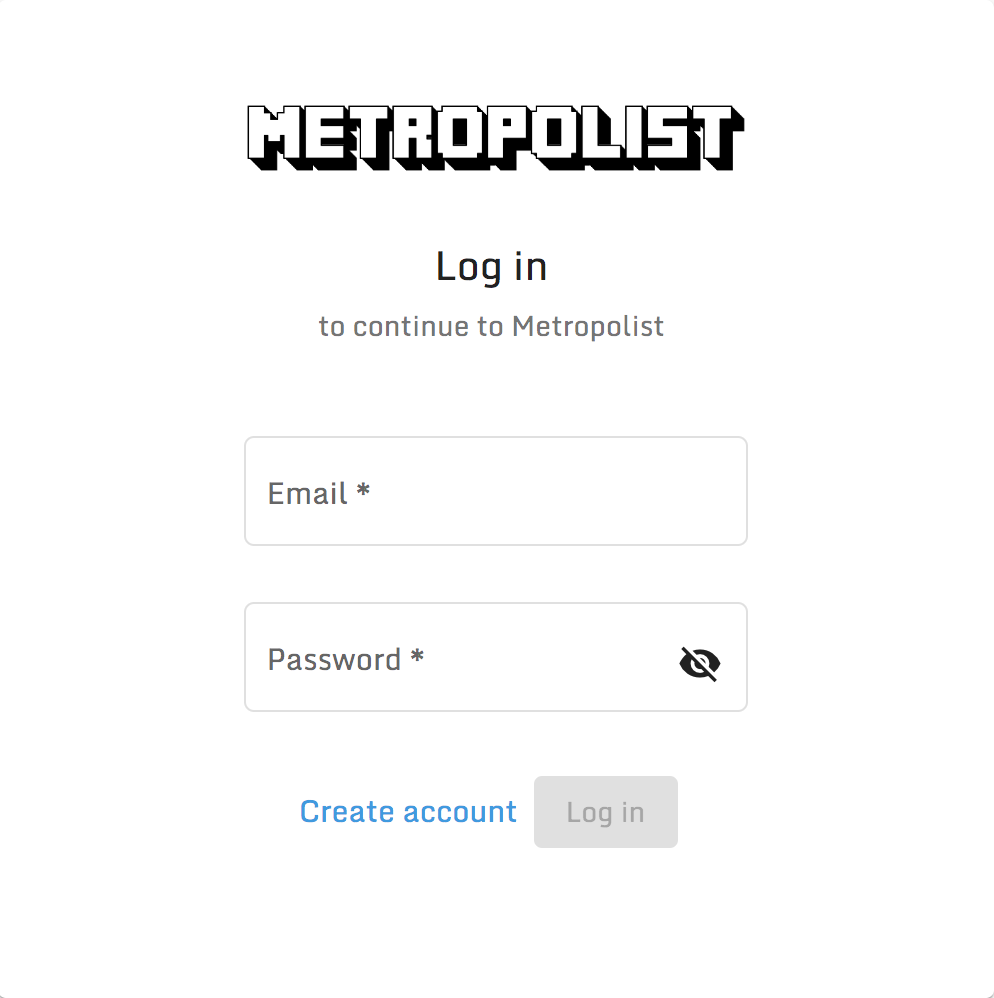
\includegraphics[width=\textwidth]{section04/assets/GUI-login-small.png}
  %   \caption{Login page}
  %   \label{fig:GUI login}
  % \end{minipage}
  % \end{figure}

  \item The ``Community'' page shows all the maps that can be viewed, which are marked by their own owners as ``isVisible.'' Besides, the user can filter maps using map name, owner's email, owner's first name, or owner's last name via the ``Filter'' on the left top corner. Figure \ref{fig:GUI community} is the interface of the ``Community'' page.

  \begin{figure}[htbp]
    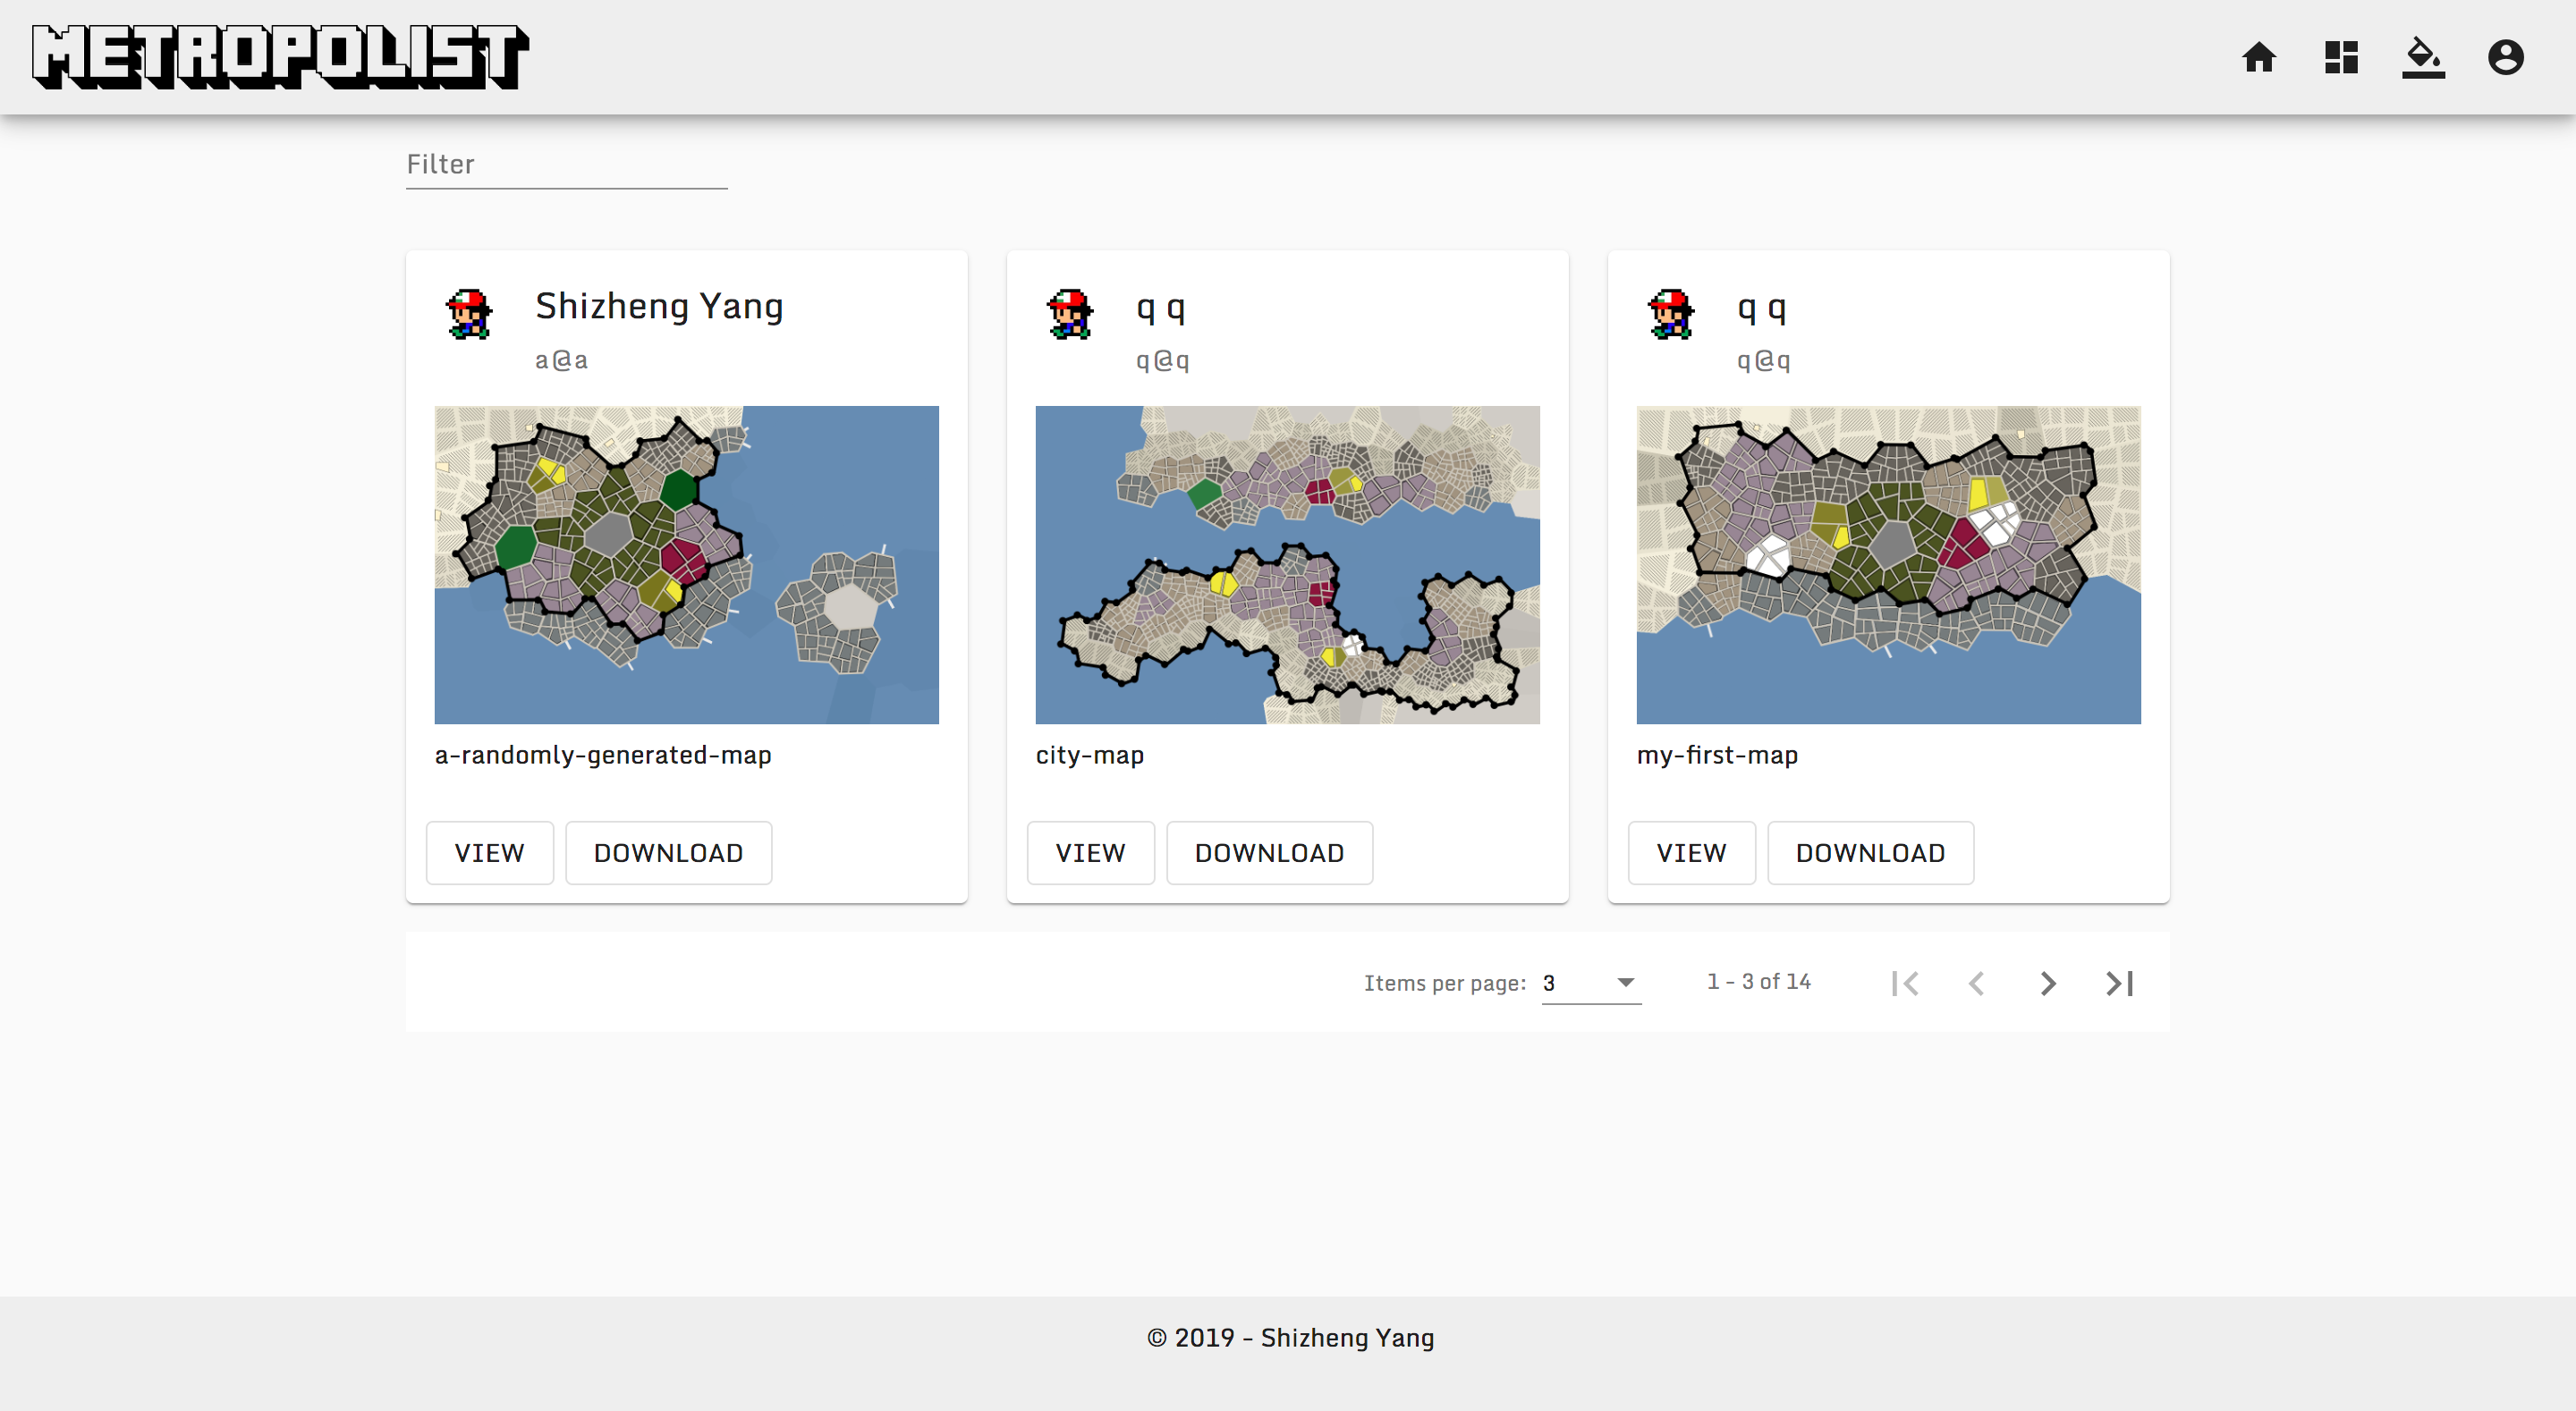
\includegraphics[width=\textwidth]{section04/assets/GUI-community.png}
    \caption{Community page}
    \label{fig:GUI community}
  \end{figure}

  \item The ``User Dashboard'' page displays all the maps belonging to the current user. The user can filter them using any information of maps via the ``Filter'' on the left top corner. The user can click on the header to perform the sorting of the corresponding map properties. Also, the user is allowed to make the map be visible or invisible by manipulating the slide of ``isVisible'', and edit, delete or download it via the three buttons in the ``Operation'' column. In addition, The button for creating a new map is in the lower right corner of the page. The user can enter a map name in the pop-up window after clicking it. Figure \ref{fig:GUI user dashboard} is the interface of the User dashboard page.

  \begin{figure}[htbp]
    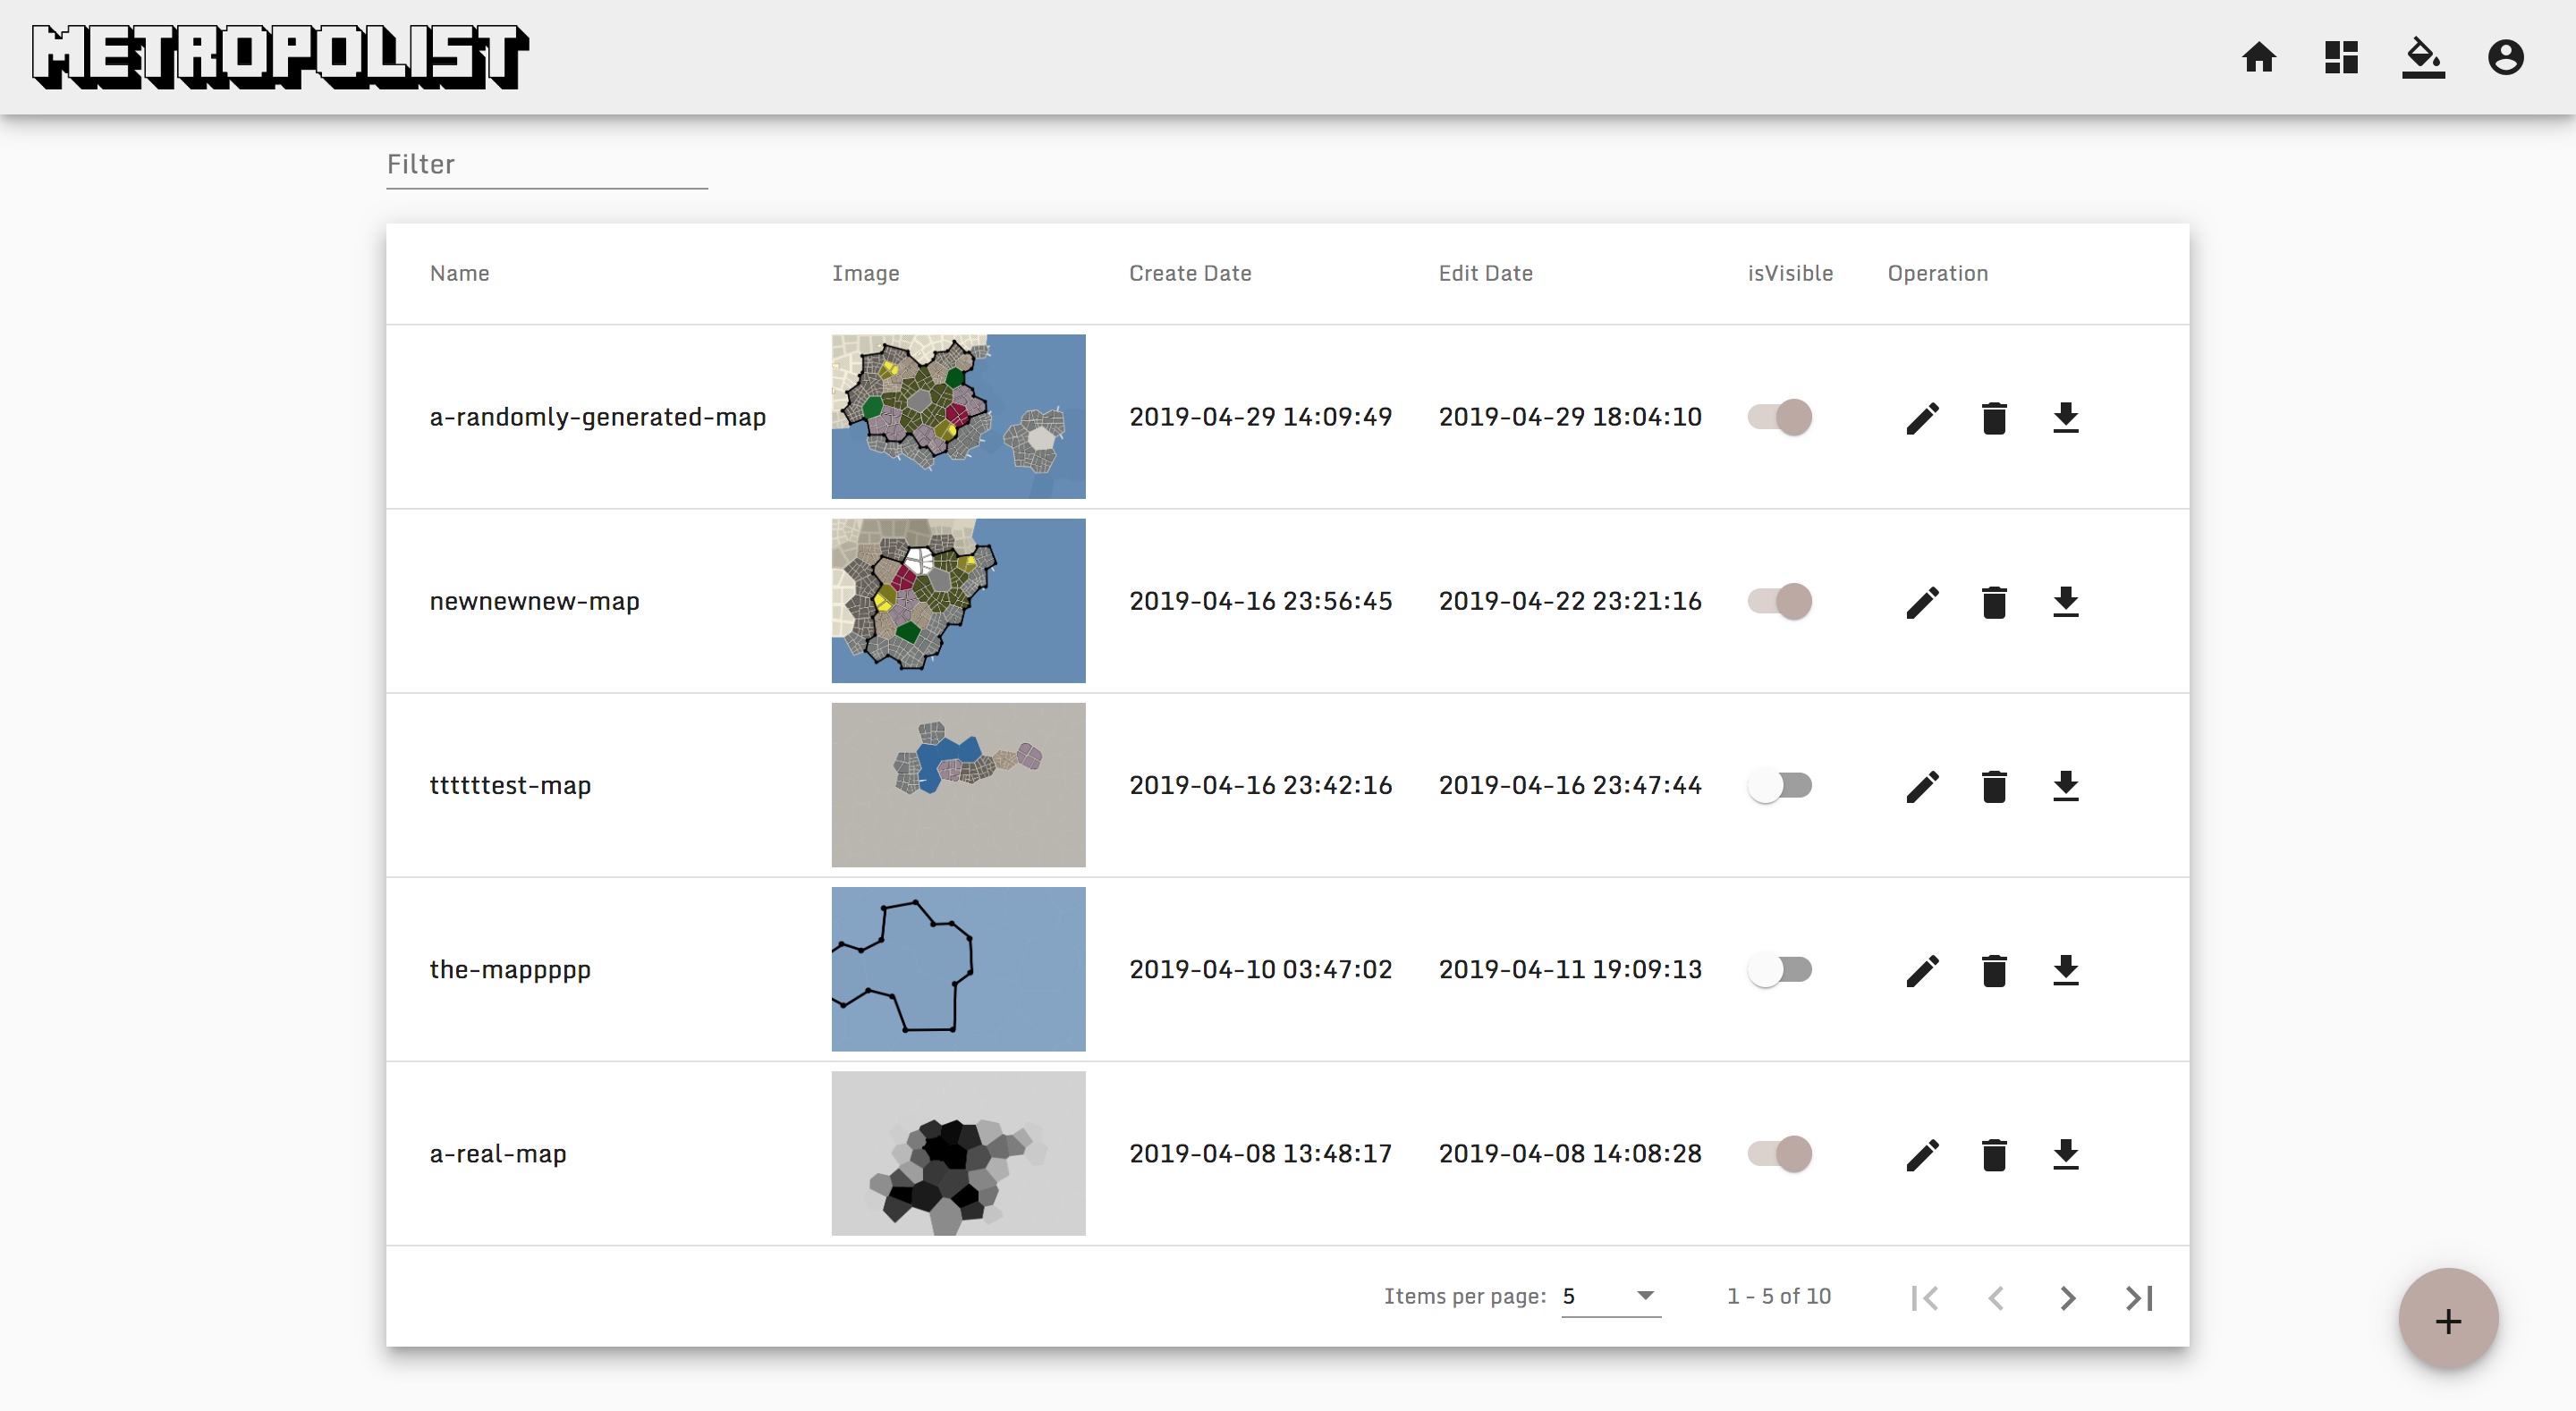
\includegraphics[width=\textwidth]{section04/assets/GUI-user.png}
    \caption{User dashboard page}
    \label{fig:GUI user dashboard}
  \end{figure}

  \item The ``Profile'' page allows the user to change his email, password, first name, or last name. By the way, before changing the password, the user must first enter the old password. After the verification is passed, the new password can be entered. Figure \ref{fig:GUI profile} is the interface of the Profile page.

  \begin{figure}[htbp]
    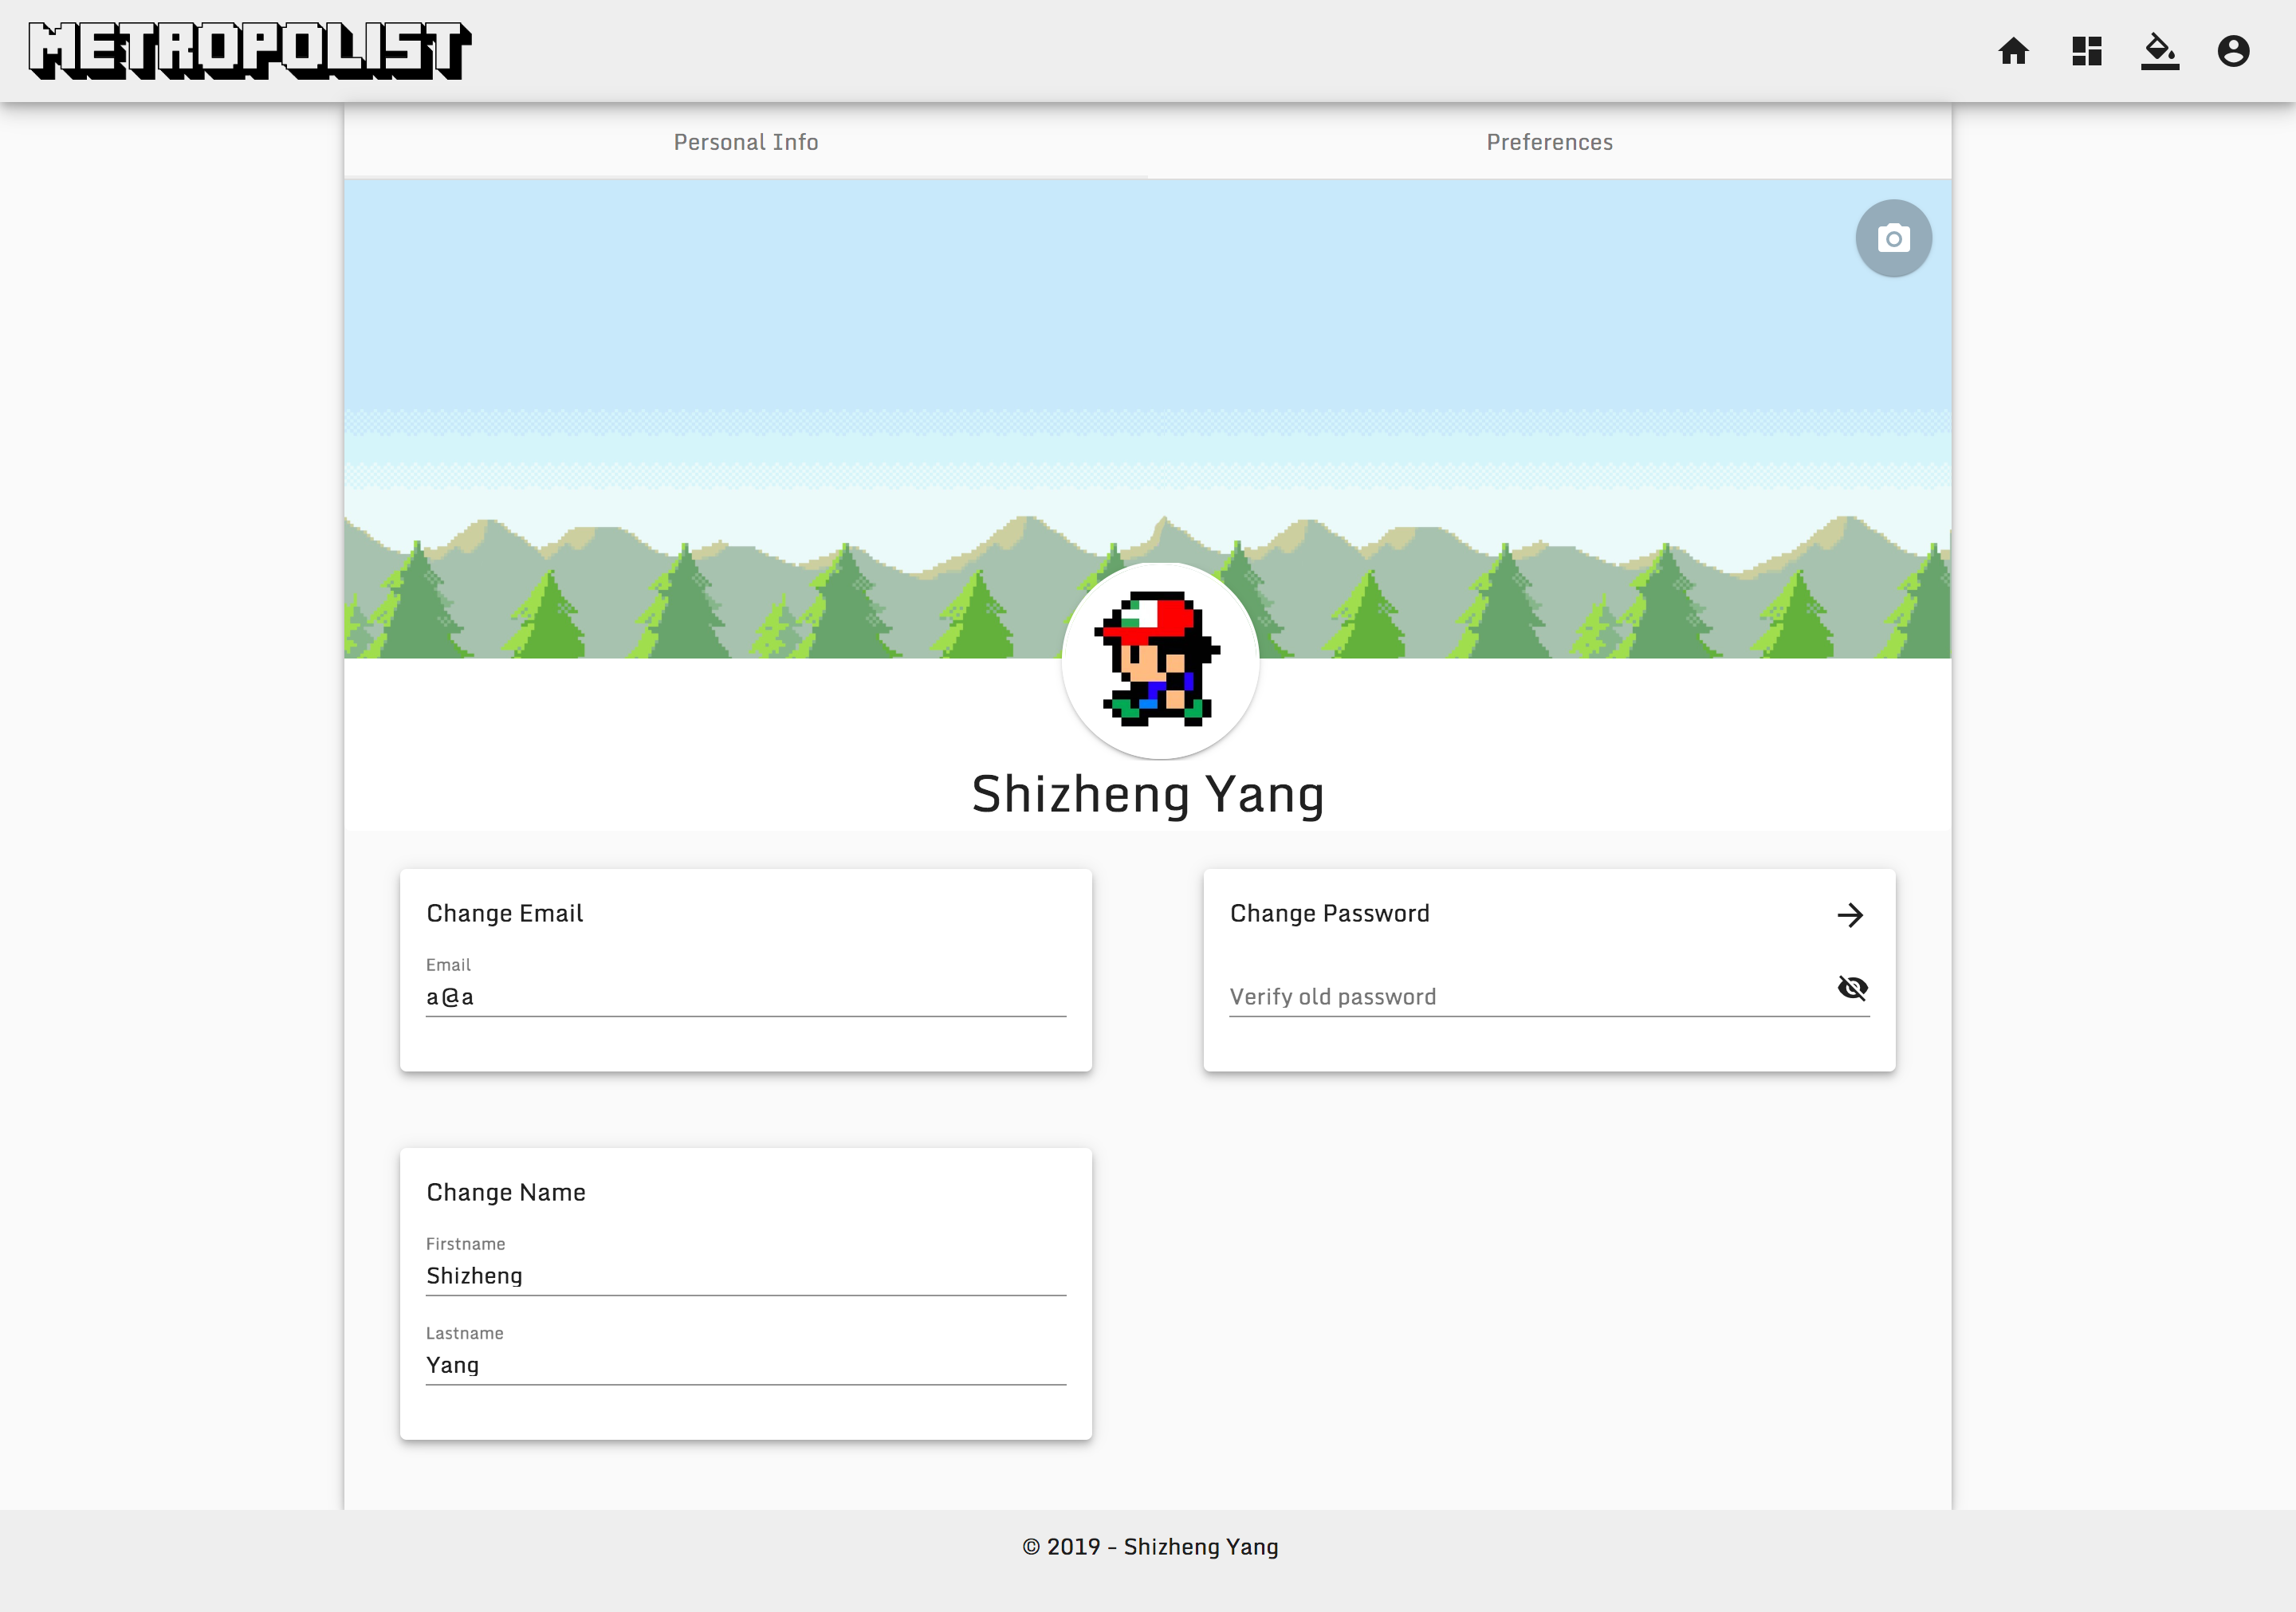
\includegraphics[width=\textwidth]{section04/assets/GUI-profile.png}
    \caption{Profile page}
    \label{fig:GUI profile}
  \end{figure}

\end{enumerate}

\subsection{Backend}
The backend consists of the server, database, and APIs. The server running on the developer's computer, the database is powered by MongoDB, and the APIs are RESTful. On this basis, we chose Express.js because it is a lightweight Node.js framework, which allows us to define routes of our application based on HTTP methods and URLs so that we can easily apply the REST API design to them very well. Also, it includes various middleware modules that we can use to perform additional tasks on the request and response.

To connect MongoDB to our Express application, we had to use an ORM to convert information from the database to a JavaScript application without SQL statements. ORM is short for Object Related Mapping, a technique that can be used to convert data among incompatible types. More specifically, ORMs mimic the actual database so we can operate within a programming language (e.g. JavaScript) without using a database query language (e.g. SQL) to interact with the database. For this application, we used Mongoose as the ORM, which is an object document modeling (ODM) layer that sits on top of the Node.js's MongoDB driver.

Figure \ref{fig:Backend Folder Structure} shows the final structure of the backend application powered by Node.js. Figure \ref{fig:Endpoints} shows a part of implemented endpoints, which are located in src/routes/index.js.

\begin{figure}[htbp]
  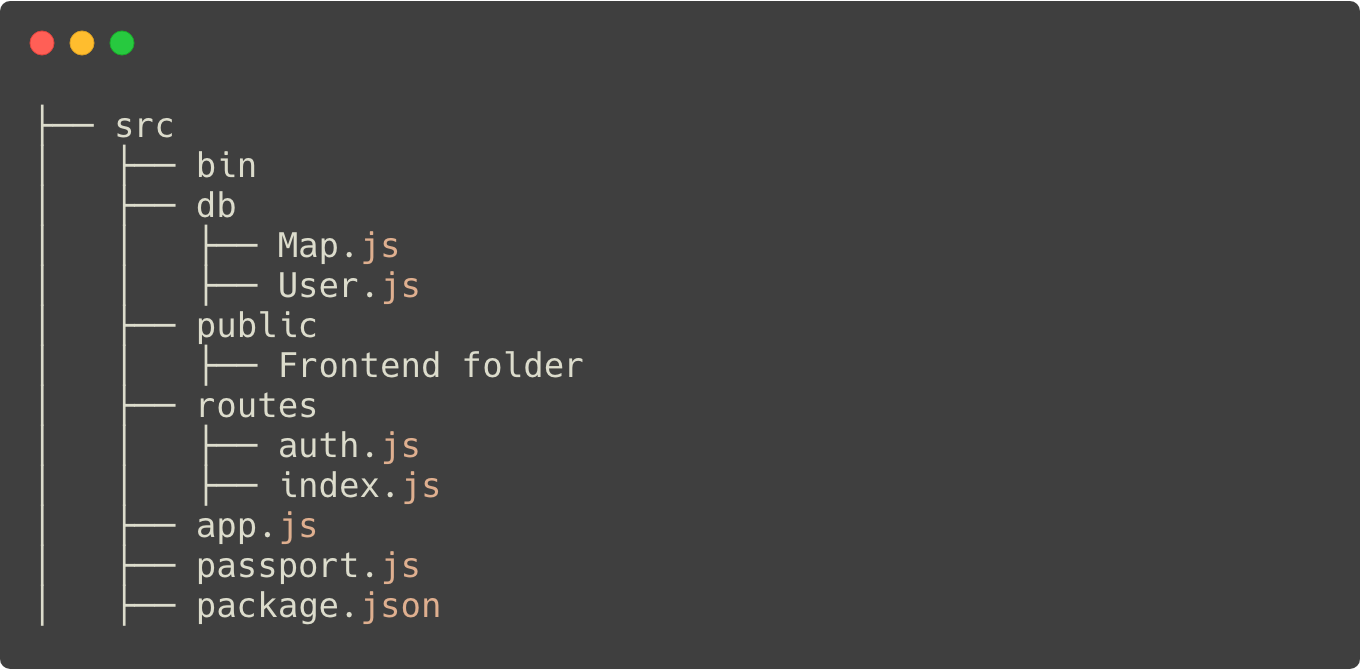
\includegraphics[width=\textwidth]{section04/assets/Backend.png}
  \caption{Backend Folder Structure}
  \label{fig:Backend Folder Structure}
\end{figure}

\begin{figure}[htbp]
  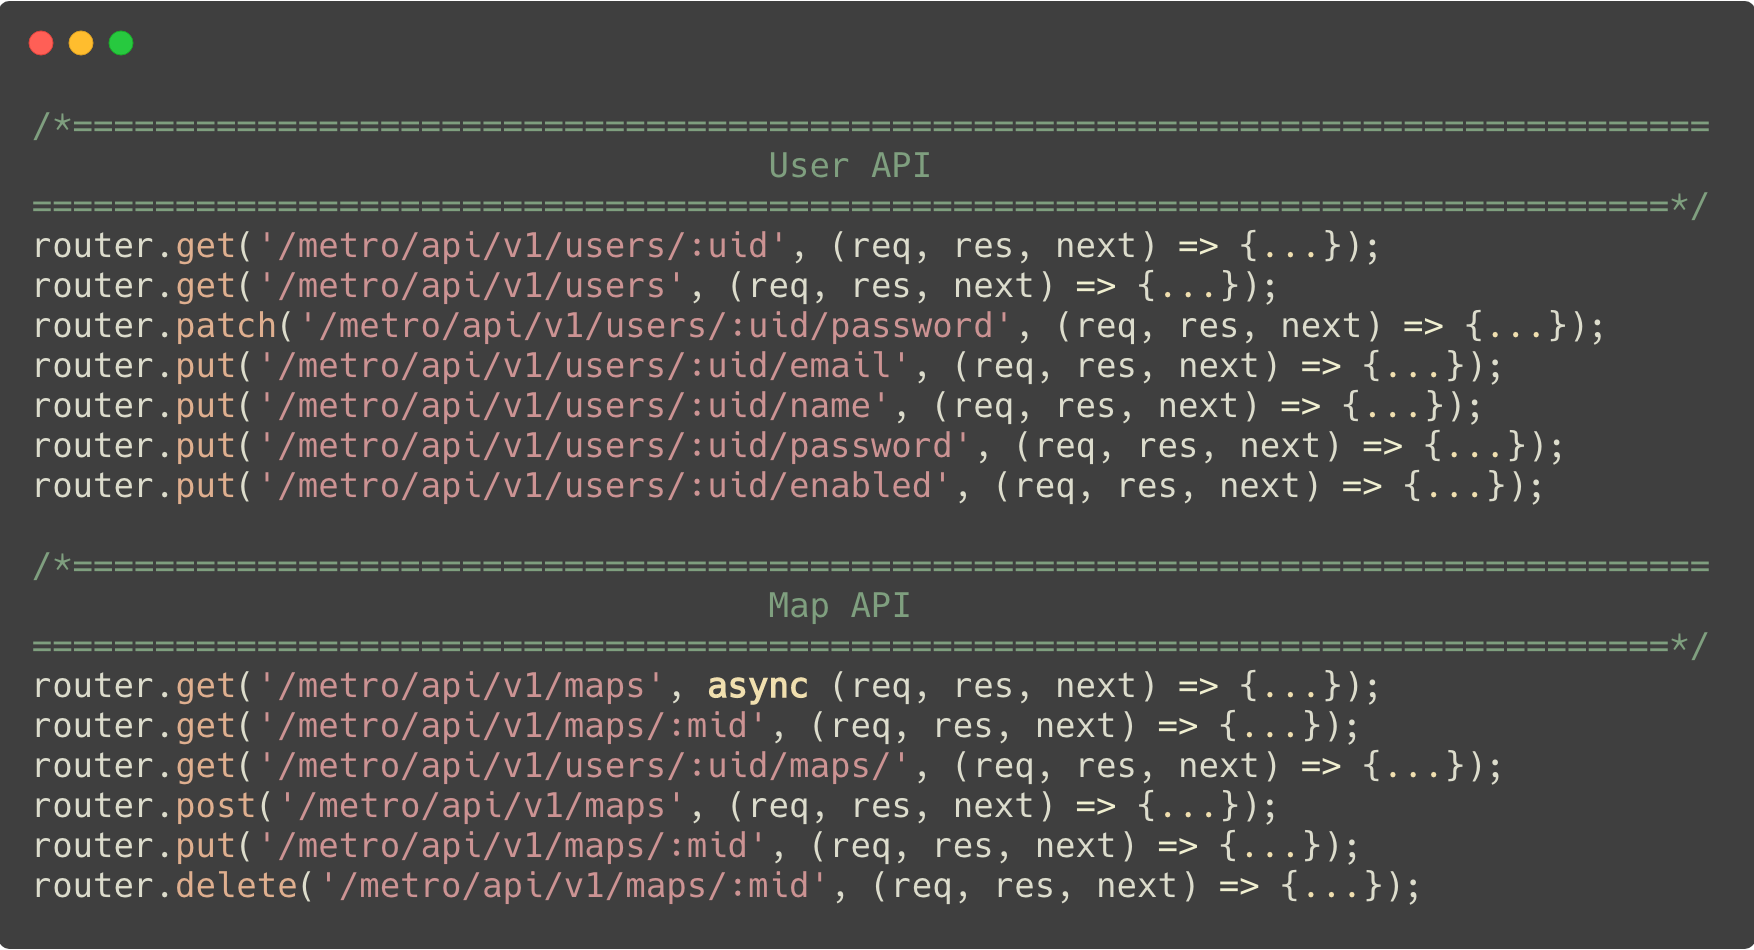
\includegraphics[width=\textwidth]{section04/assets/Endpoints.png}
  \caption{Endpoints}
  \label{fig:Endpoints}
\end{figure}

\subsection{Map Generator}
\subsubsection{Polygons}
The first step is to render some polygons (cells). As we mentioned before in the design phase, we used the d3.voronoi library to implement Steven J. Fortune’s algorithm for computing the Voronoi diagram or Delaunay triangulation of a set of two-dimensional points. Figure \ref{fig:Voronoi polygons} is an example of 100 dots and the corresponding 100 polygons:

As we can see the tessellation of these random points is irregulars. In the sense that ratio between the largest and smallest region is overly large. To reduce this variance and obtain a more regular partition, we used a variant of Lloyd relaxation, also known as Voronoi iteration or relaxation, which has the effect of making the polygons evenly distributed. Lloyd relaxation replaces each point by the centroid of its polygon. The more iterations, the more regular the polygons get. Figure \ref{fig:Voronoi relaxed polygons} is the result after running approximate Lloyd relaxation 5 times:

\begin{figure}
\centering
  \begin{subfigure}{.5\textwidth}
    \centering
    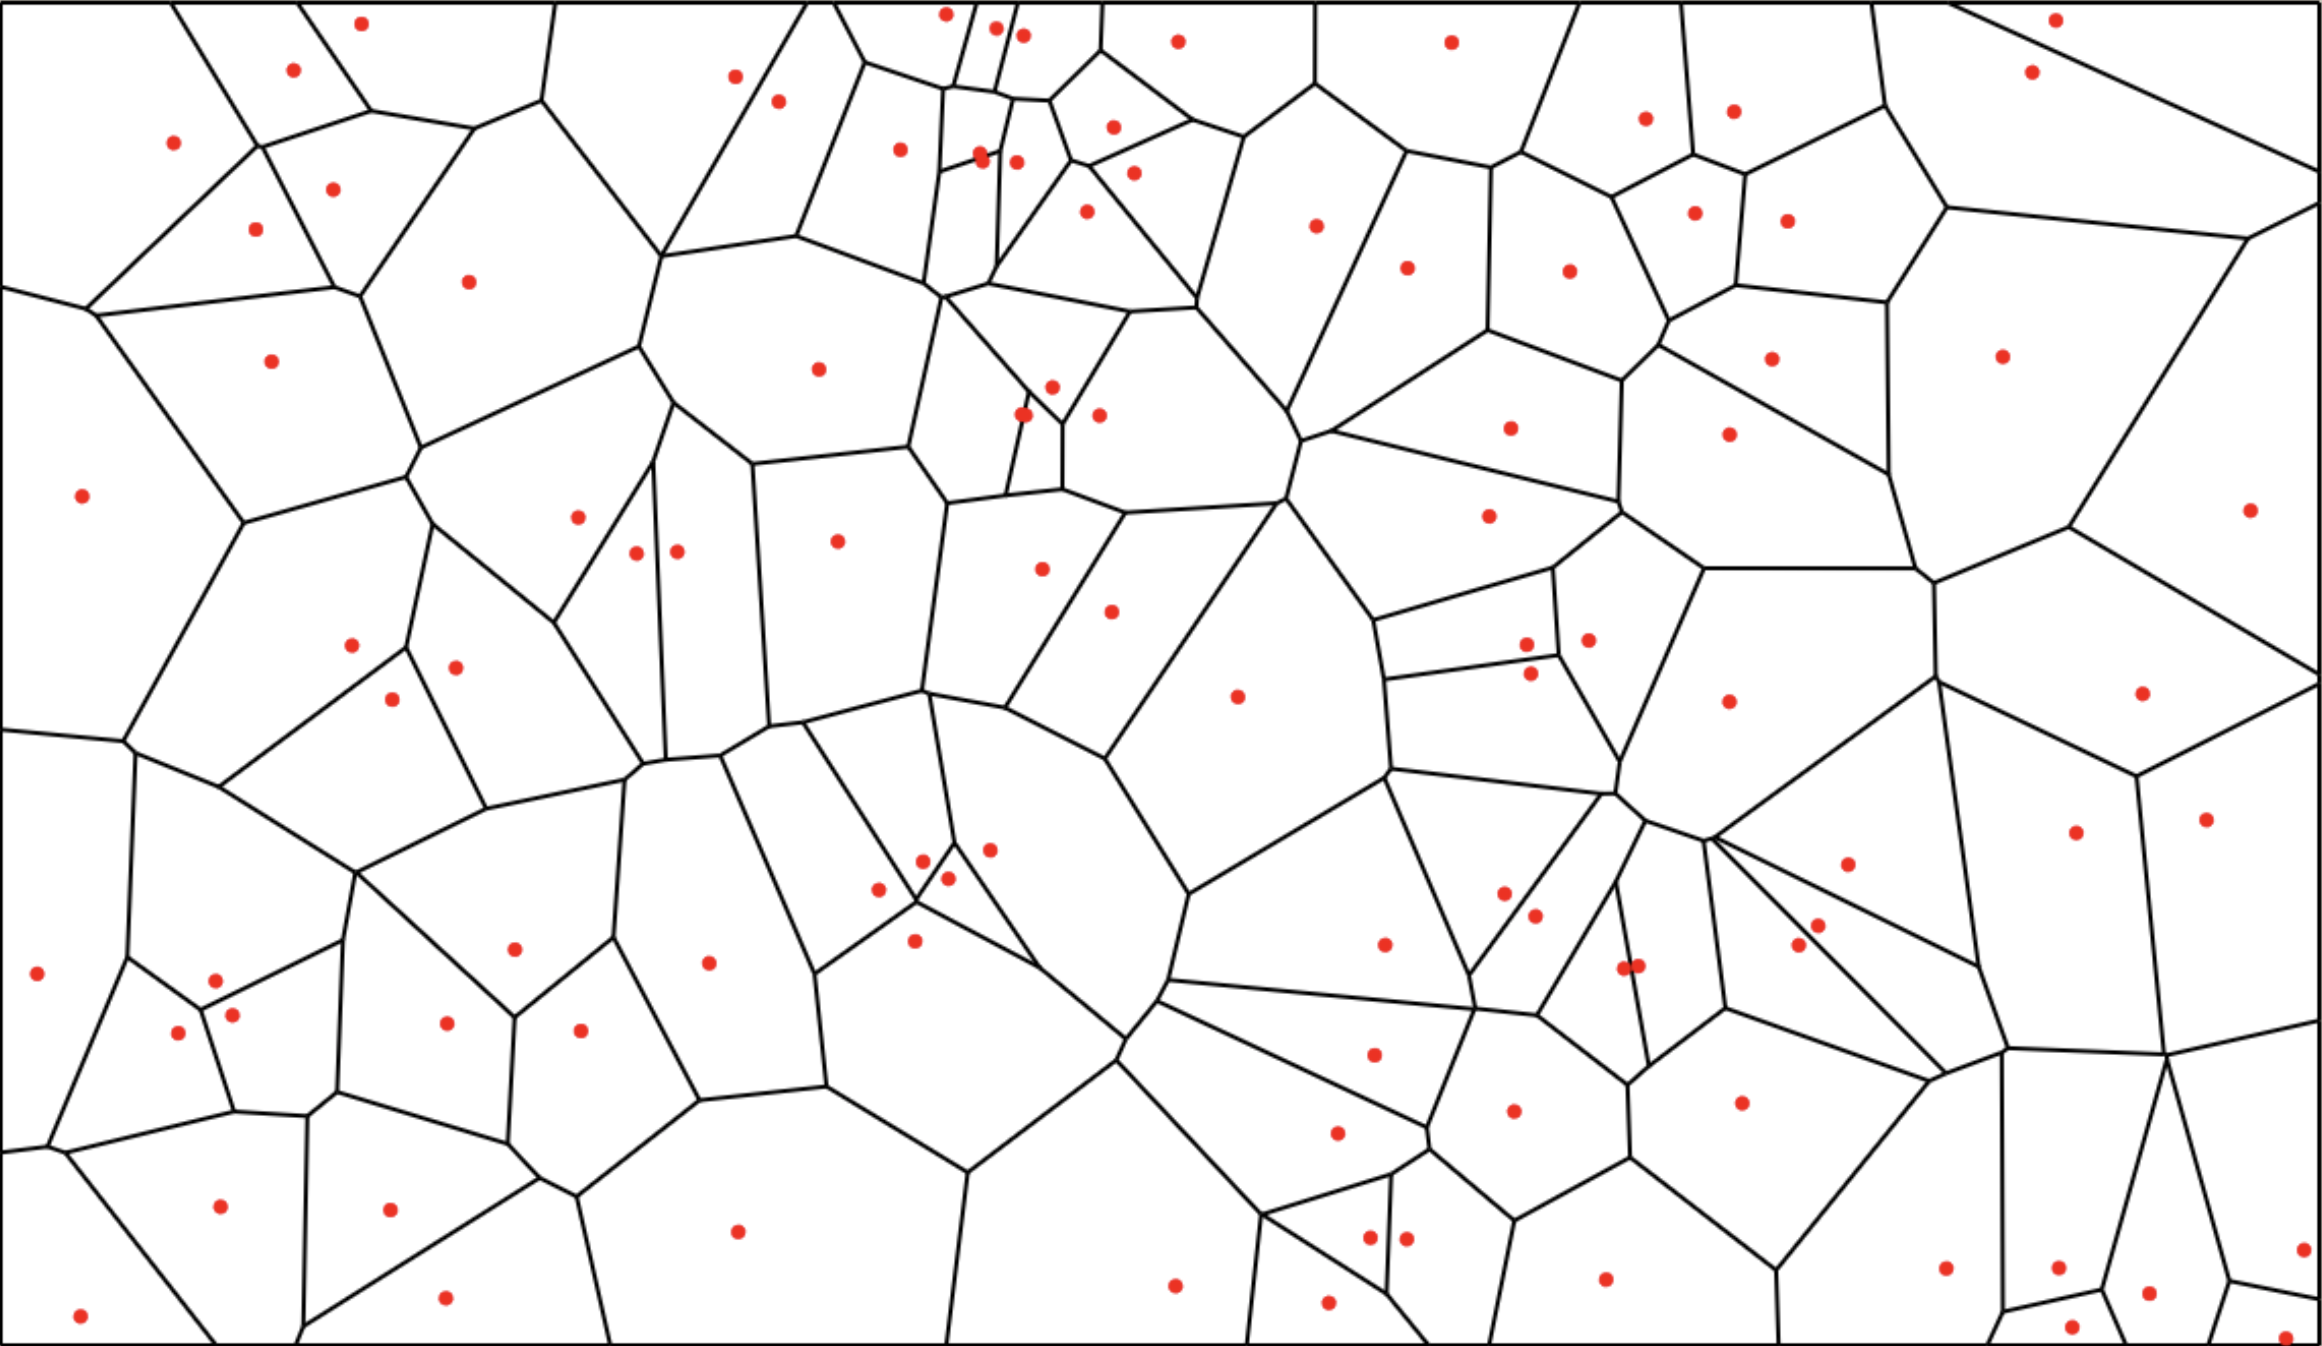
\includegraphics[width=.99\textwidth]{section04/assets/Map-voronoi.png}
    \caption{Before relaxation}
    \label{fig:Voronoi polygons}
  \end{subfigure}%
  \begin{subfigure}{.5\textwidth}
    \centering
    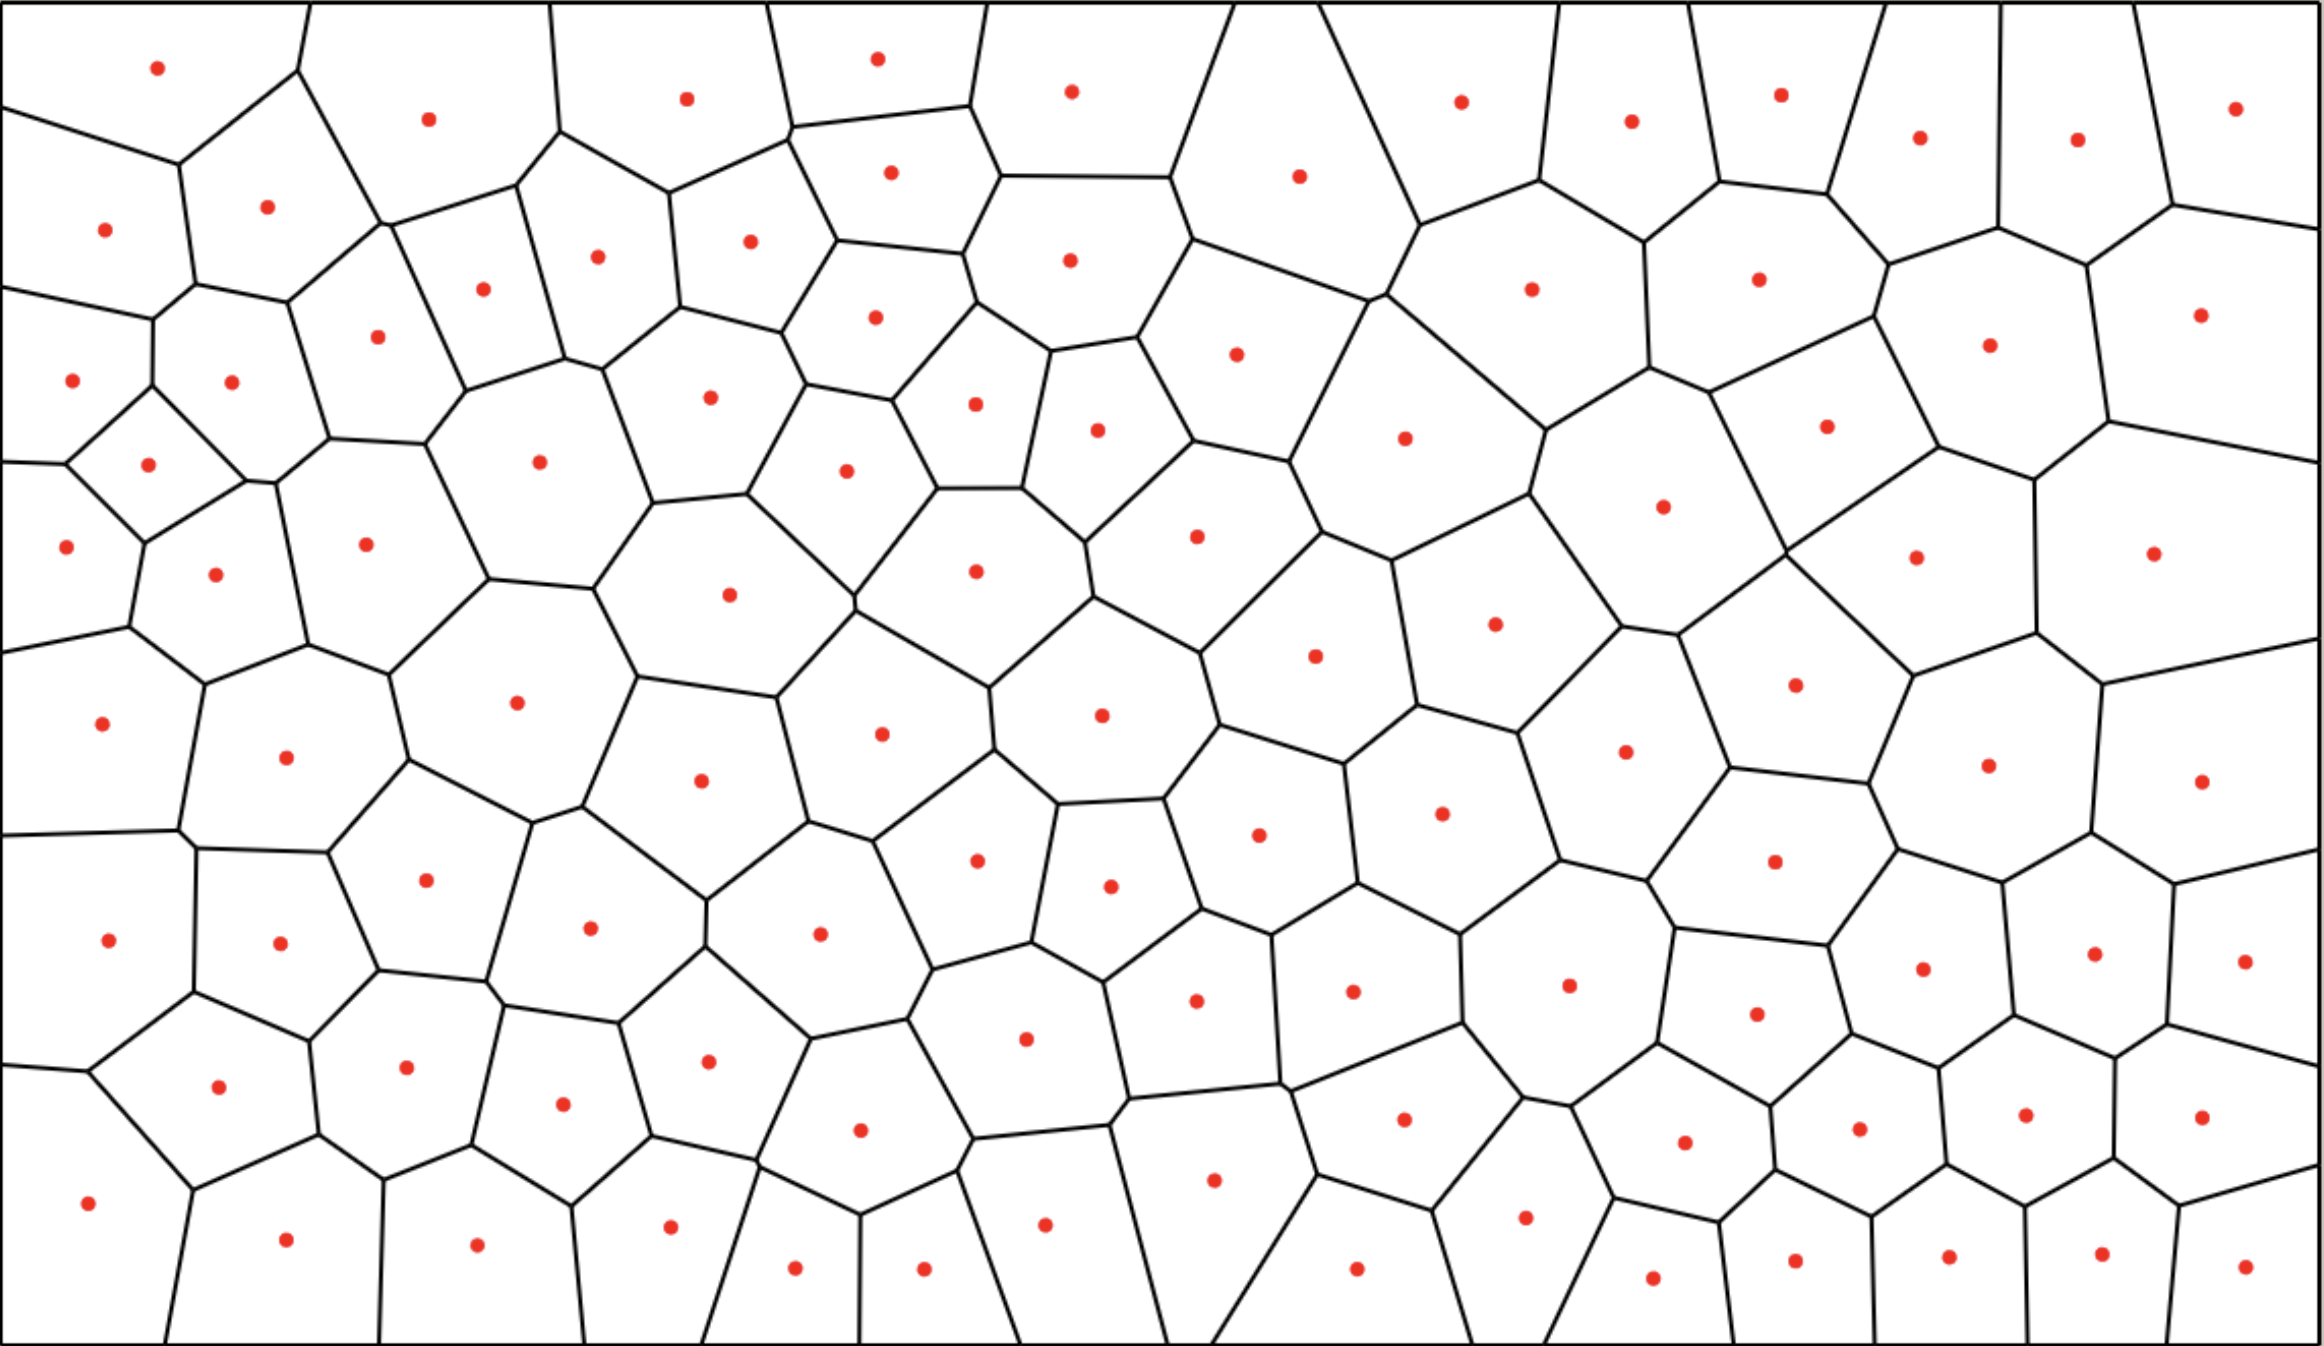
\includegraphics[width=.99\textwidth]{section04/assets/Map-voronoi-relaxation.png}
    \caption{After 5 times of relaxation}
    \label{fig:Voronoi relaxed polygons}
  \end{subfigure}
  \caption{Voronoi polygons before relaxation and after relaxation}
  \label{fig:Voronoi polygons before and after Lloyd relaxation}
\end{figure}

\subsubsection{Elevation}
As we mentioned in the map generator design phase, the map should include a height layer, so we introduced the concept of ``elevation.'' We called the dots that generate polygons as sites, and each site corresponds to a polygon. Then we derived the sites object from the d3.voronoi object, and assigned the ``elevation'' property to it, whose value is normalized to the range 0..1. Before making the height map, we defined the waterline, whose value is also normalized to the range 0..1. If the value of elevation is greater than the waterline, the polygon represented by the site is a land element. Otherwise, it is water. Also, for viewing the map, darker colors denote higher elevations. As the waterline rises, the land with lower altitudes are flooded and become water. So in the beginning, we set all the polygons to be land and have an initial elevation that is 0.35. If the user wants to create water, then he should manually edit them. Figure \ref{fig:Height Map} is an example that divides the world into the land and water polygons:

\begin{figure}[htbp]
  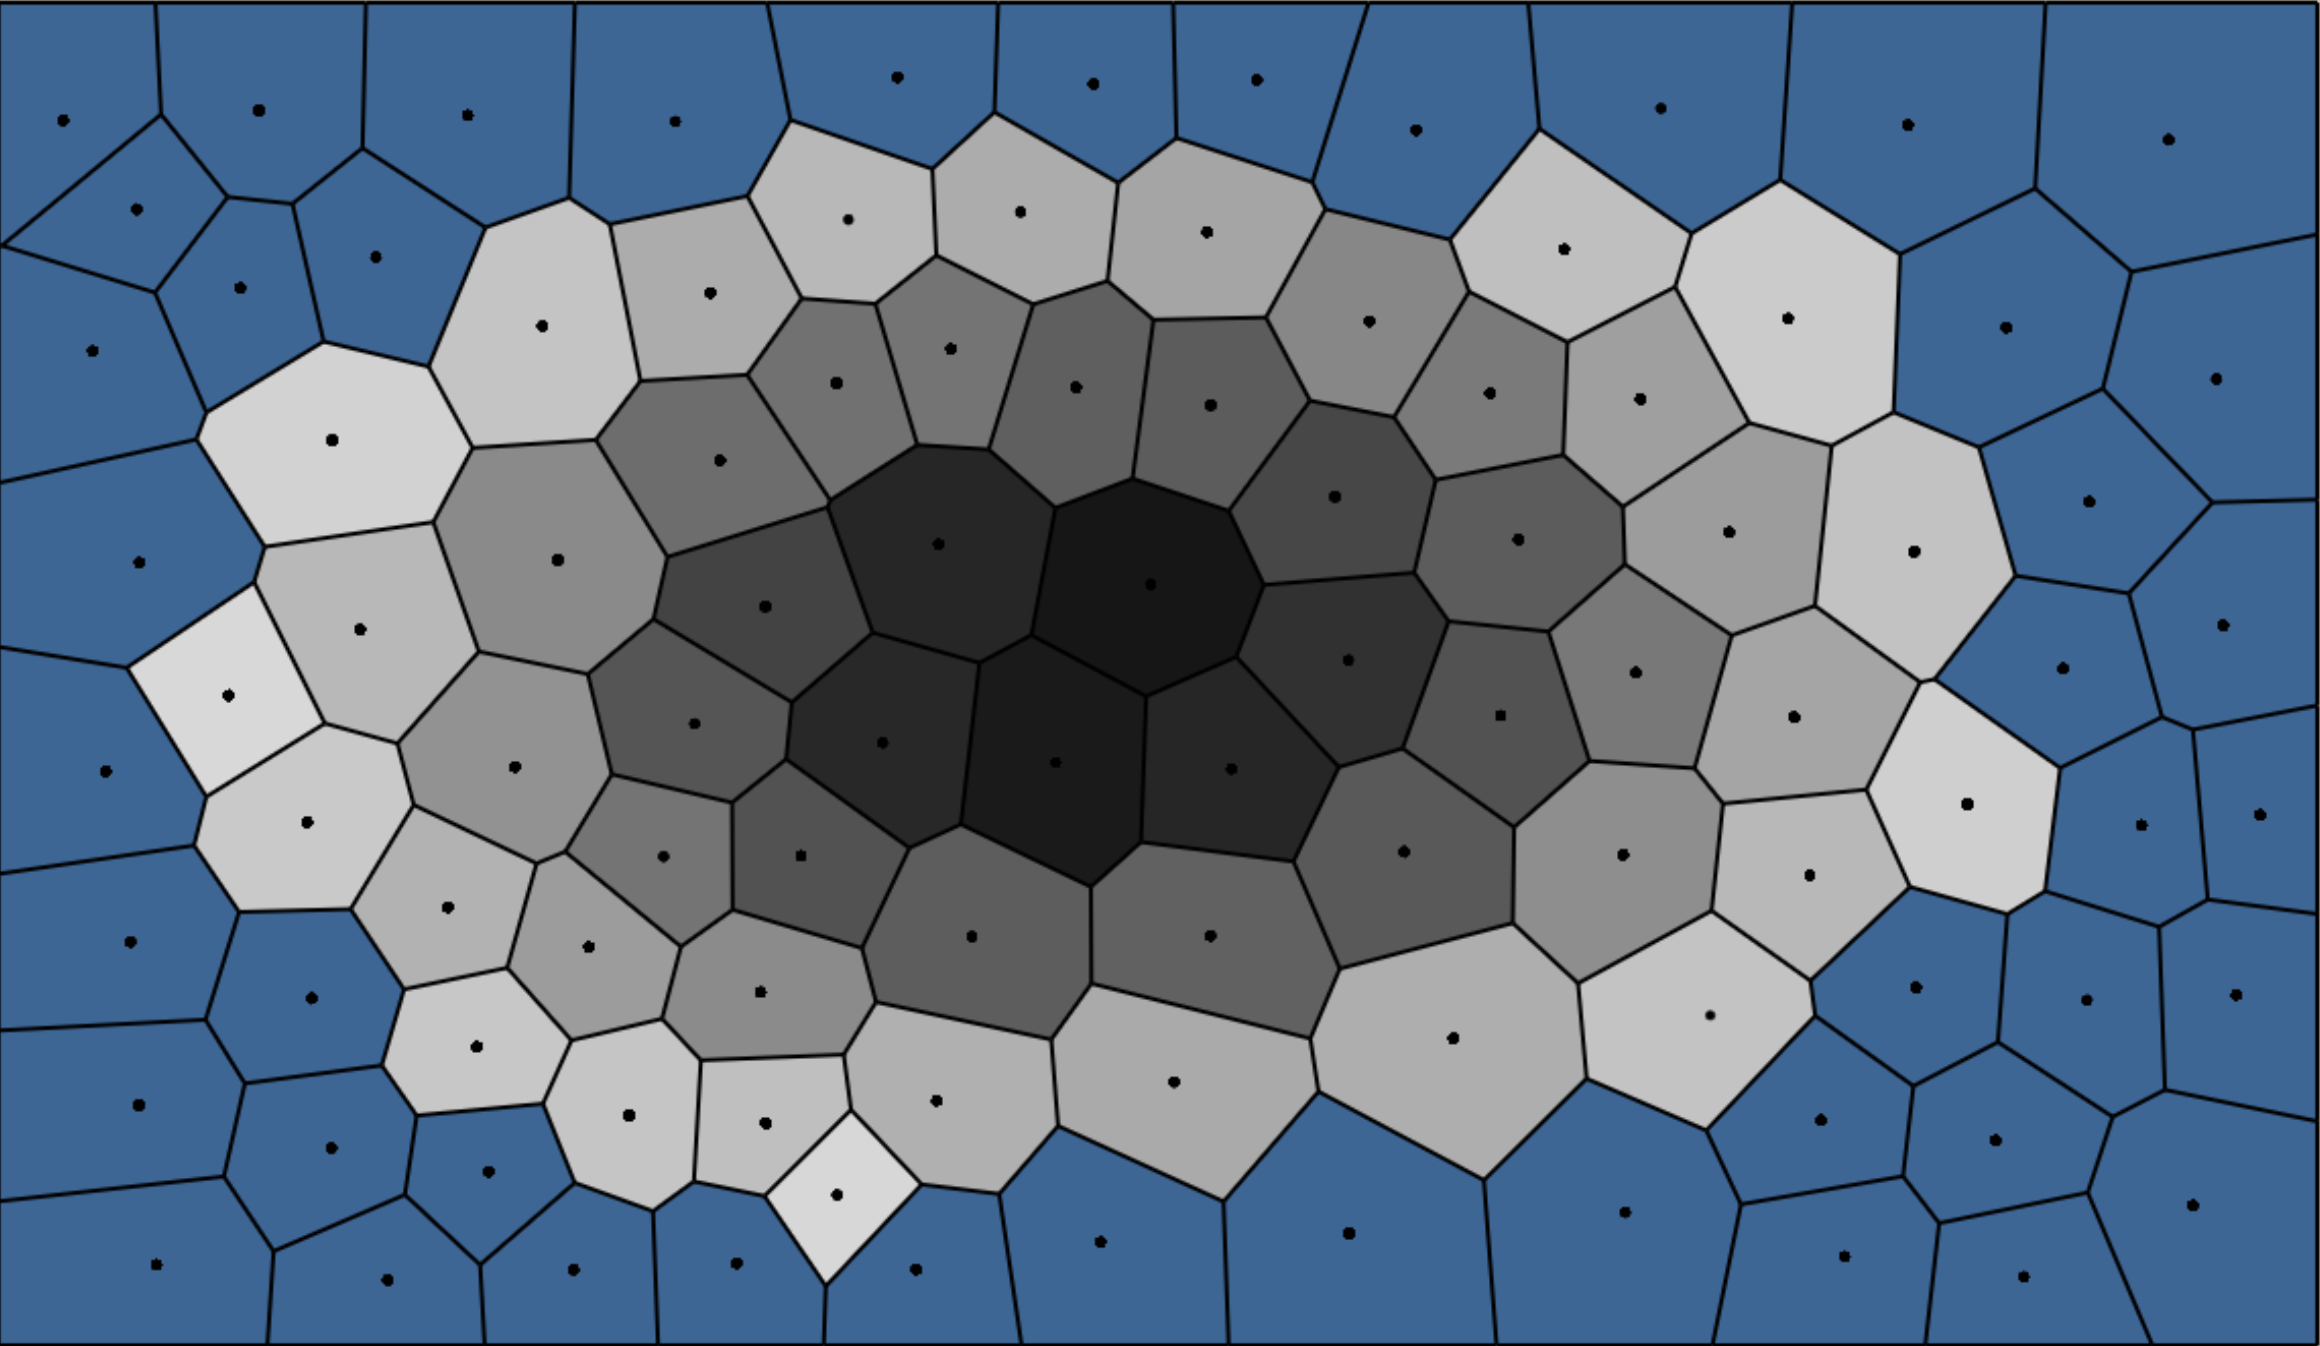
\includegraphics[width=\textwidth]{section04/assets/Map-heightmap.png}
  \caption{The land surrounded by water}
  \label{fig:Height Map}
\end{figure}

\subsubsection{Contour Lines}
We calculated the contour lines of the map, which are determined by the site elevations. The calculation of the contour lines is based on the Delaunay triangulation, which is related to the Voronoi diagram. Every triangle in the Delaunay triangulation corresponds to a polygon corner in the Voronoi diagram. Every polygon in the Voronoi diagram corresponds to a corner of a Delaunay triangle. Every edge in the Delaunay graph corresponds to an edge in the Voronoi graph. We computed these triangles directly from d3.voronoi.triangles(). Figure \ref{fig:Delaunay triangulation} is the Delaunay triangulation graph based on the Voronoi diagram after relaxation.

\begin{figure}[htbp]
  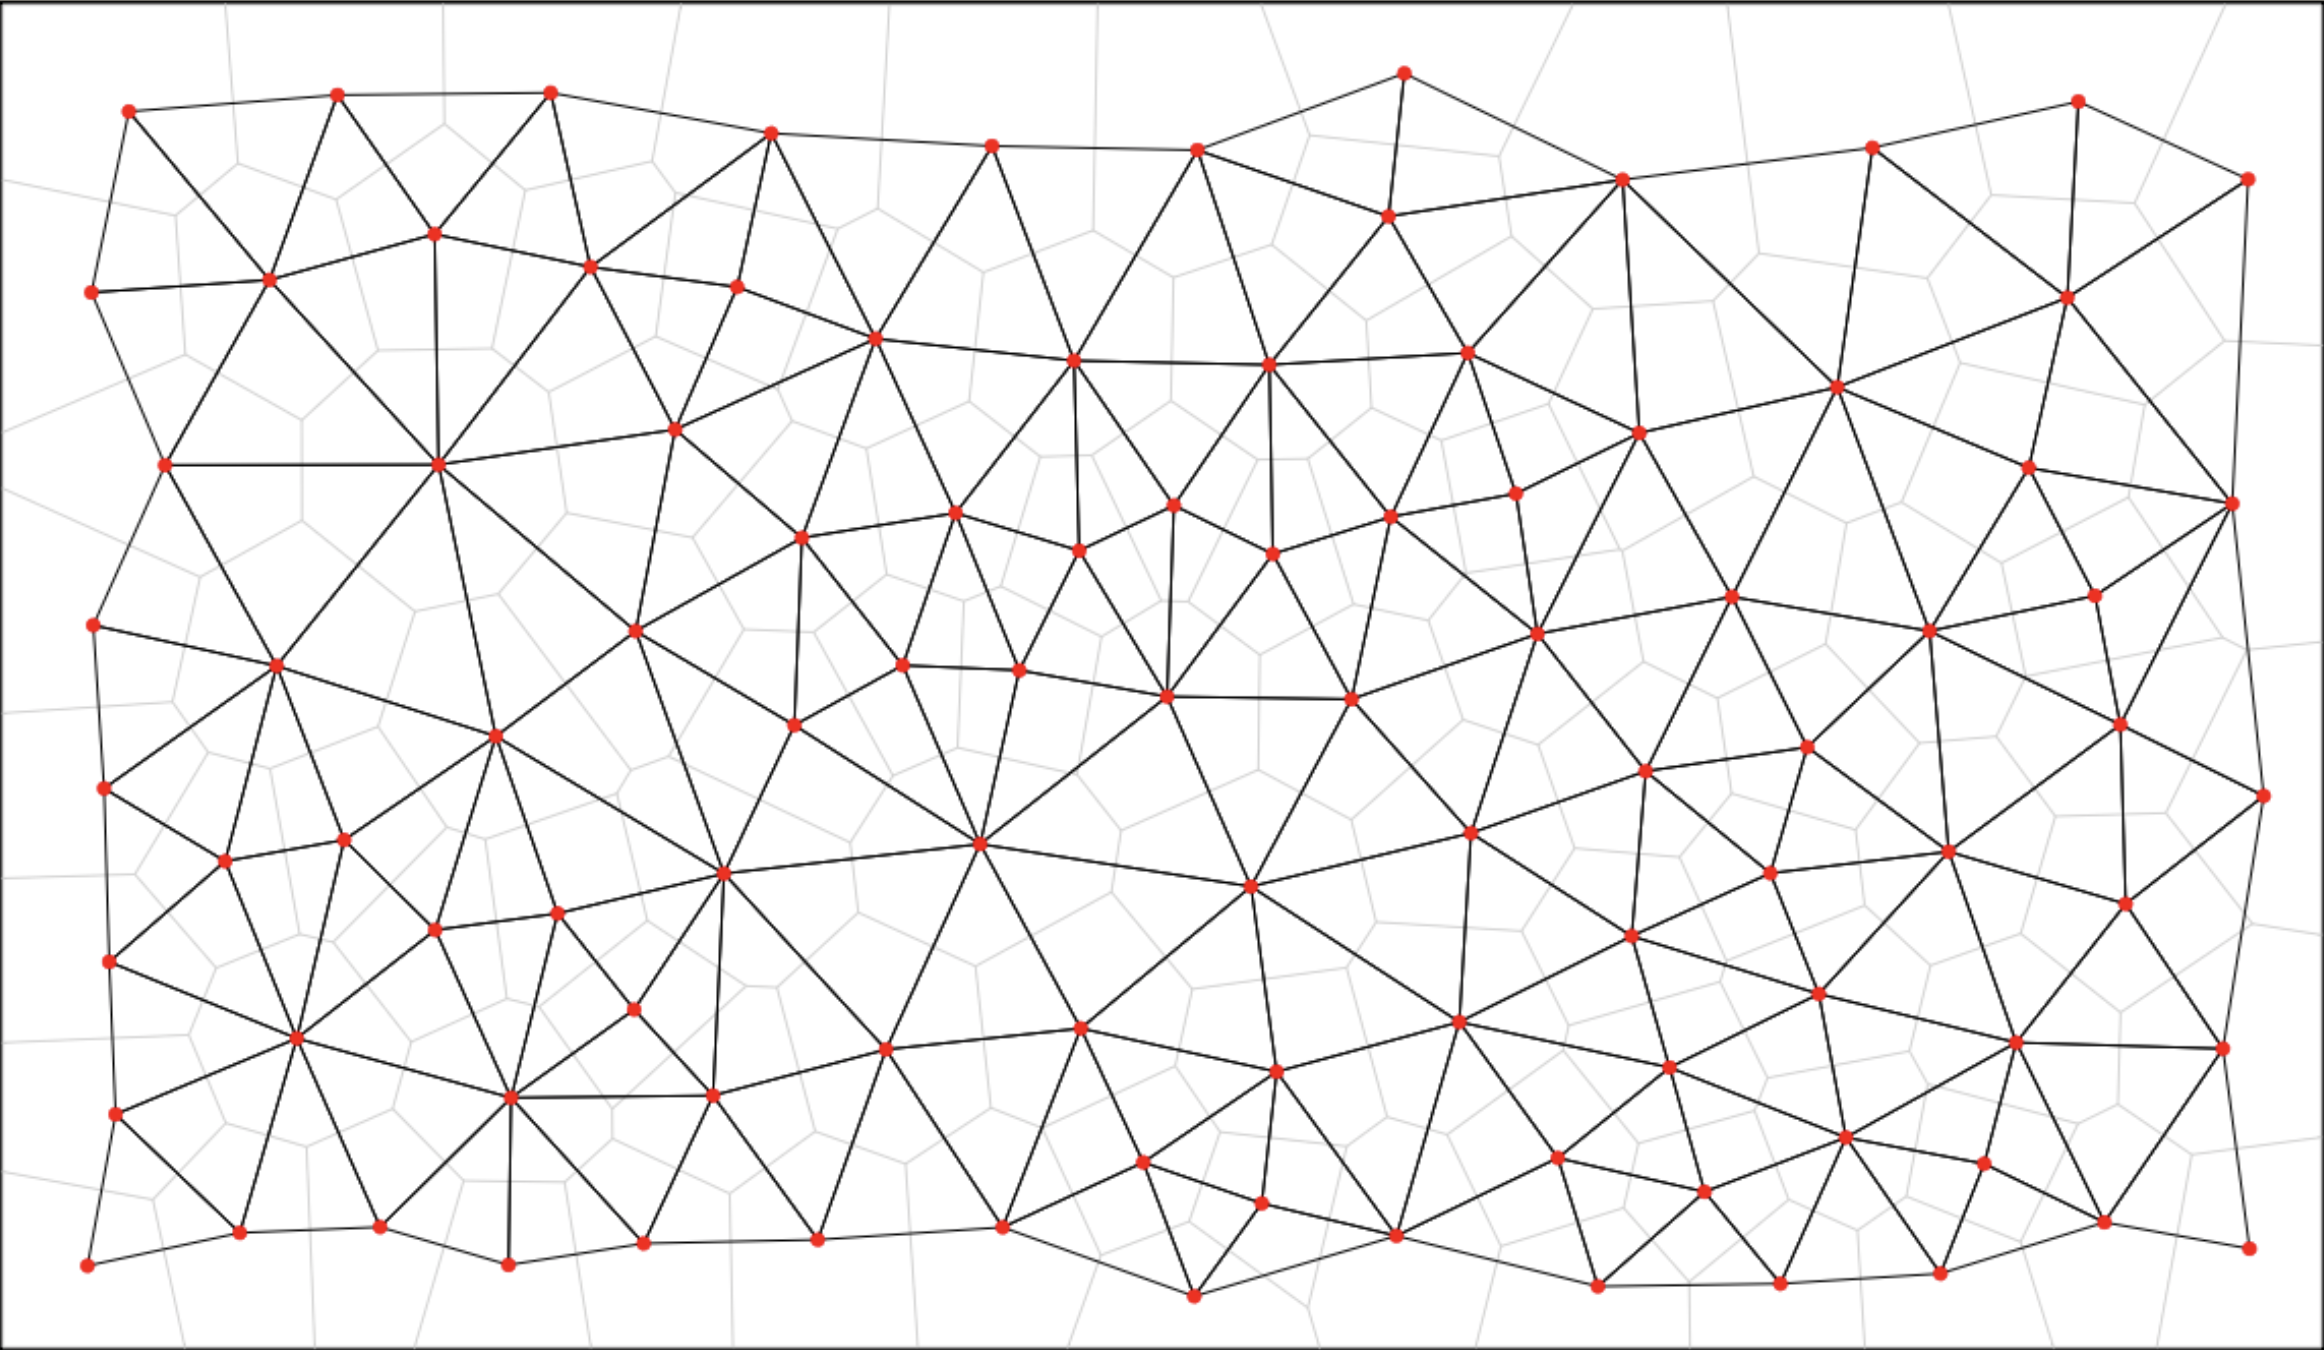
\includegraphics[width=\textwidth]{section04/assets/Map-delaunay-triangulation.png}
  \caption{Delaunay triangulation}
  \label{fig:Delaunay triangulation}
\end{figure}

These triangles link to every site, and each site has an ``elevation'' attribute. We set an elevation value between 0 and 1, and then looped over every edge of every Delaunay triangle. If this value is between the elevation values of the two sites to which it is connected, we marked the point represented by this value and then connected all such points. This process is given in pseudocode form in Algorithm \ref{alg:draw contourline}.

\begin{algorithm}
\caption{Draw contour lines for elevation X}
\label{alg:draw contourline}
\begin{algorithmic}
\REQUIRE $X \geq 0 \wedge X \leq 1$
\FOR{every triangle $T$}
\FOR{every edge $E_1$, $E_2$ in $T$}
\IF{$X \geq \mathbf{elevation}(E_1) \&\& X \leq \mathbf{elevation}(E_2)$}
\STATE Draw a line from $E_1$ to $E_2$
\ENDIF
\ENDFOR
\ENDFOR
\end{algorithmic}
\end{algorithm}

We expected the user to edit the terrain contour lines by using the tools we provided. Figure \ref{fig:contour line} gives an example that draws four contour lines based on the value of waterline (blue) and several elevation values: 0.25 (red), 0.5 (green), and 0.75 (yellow).

\begin{figure}[htbp]
  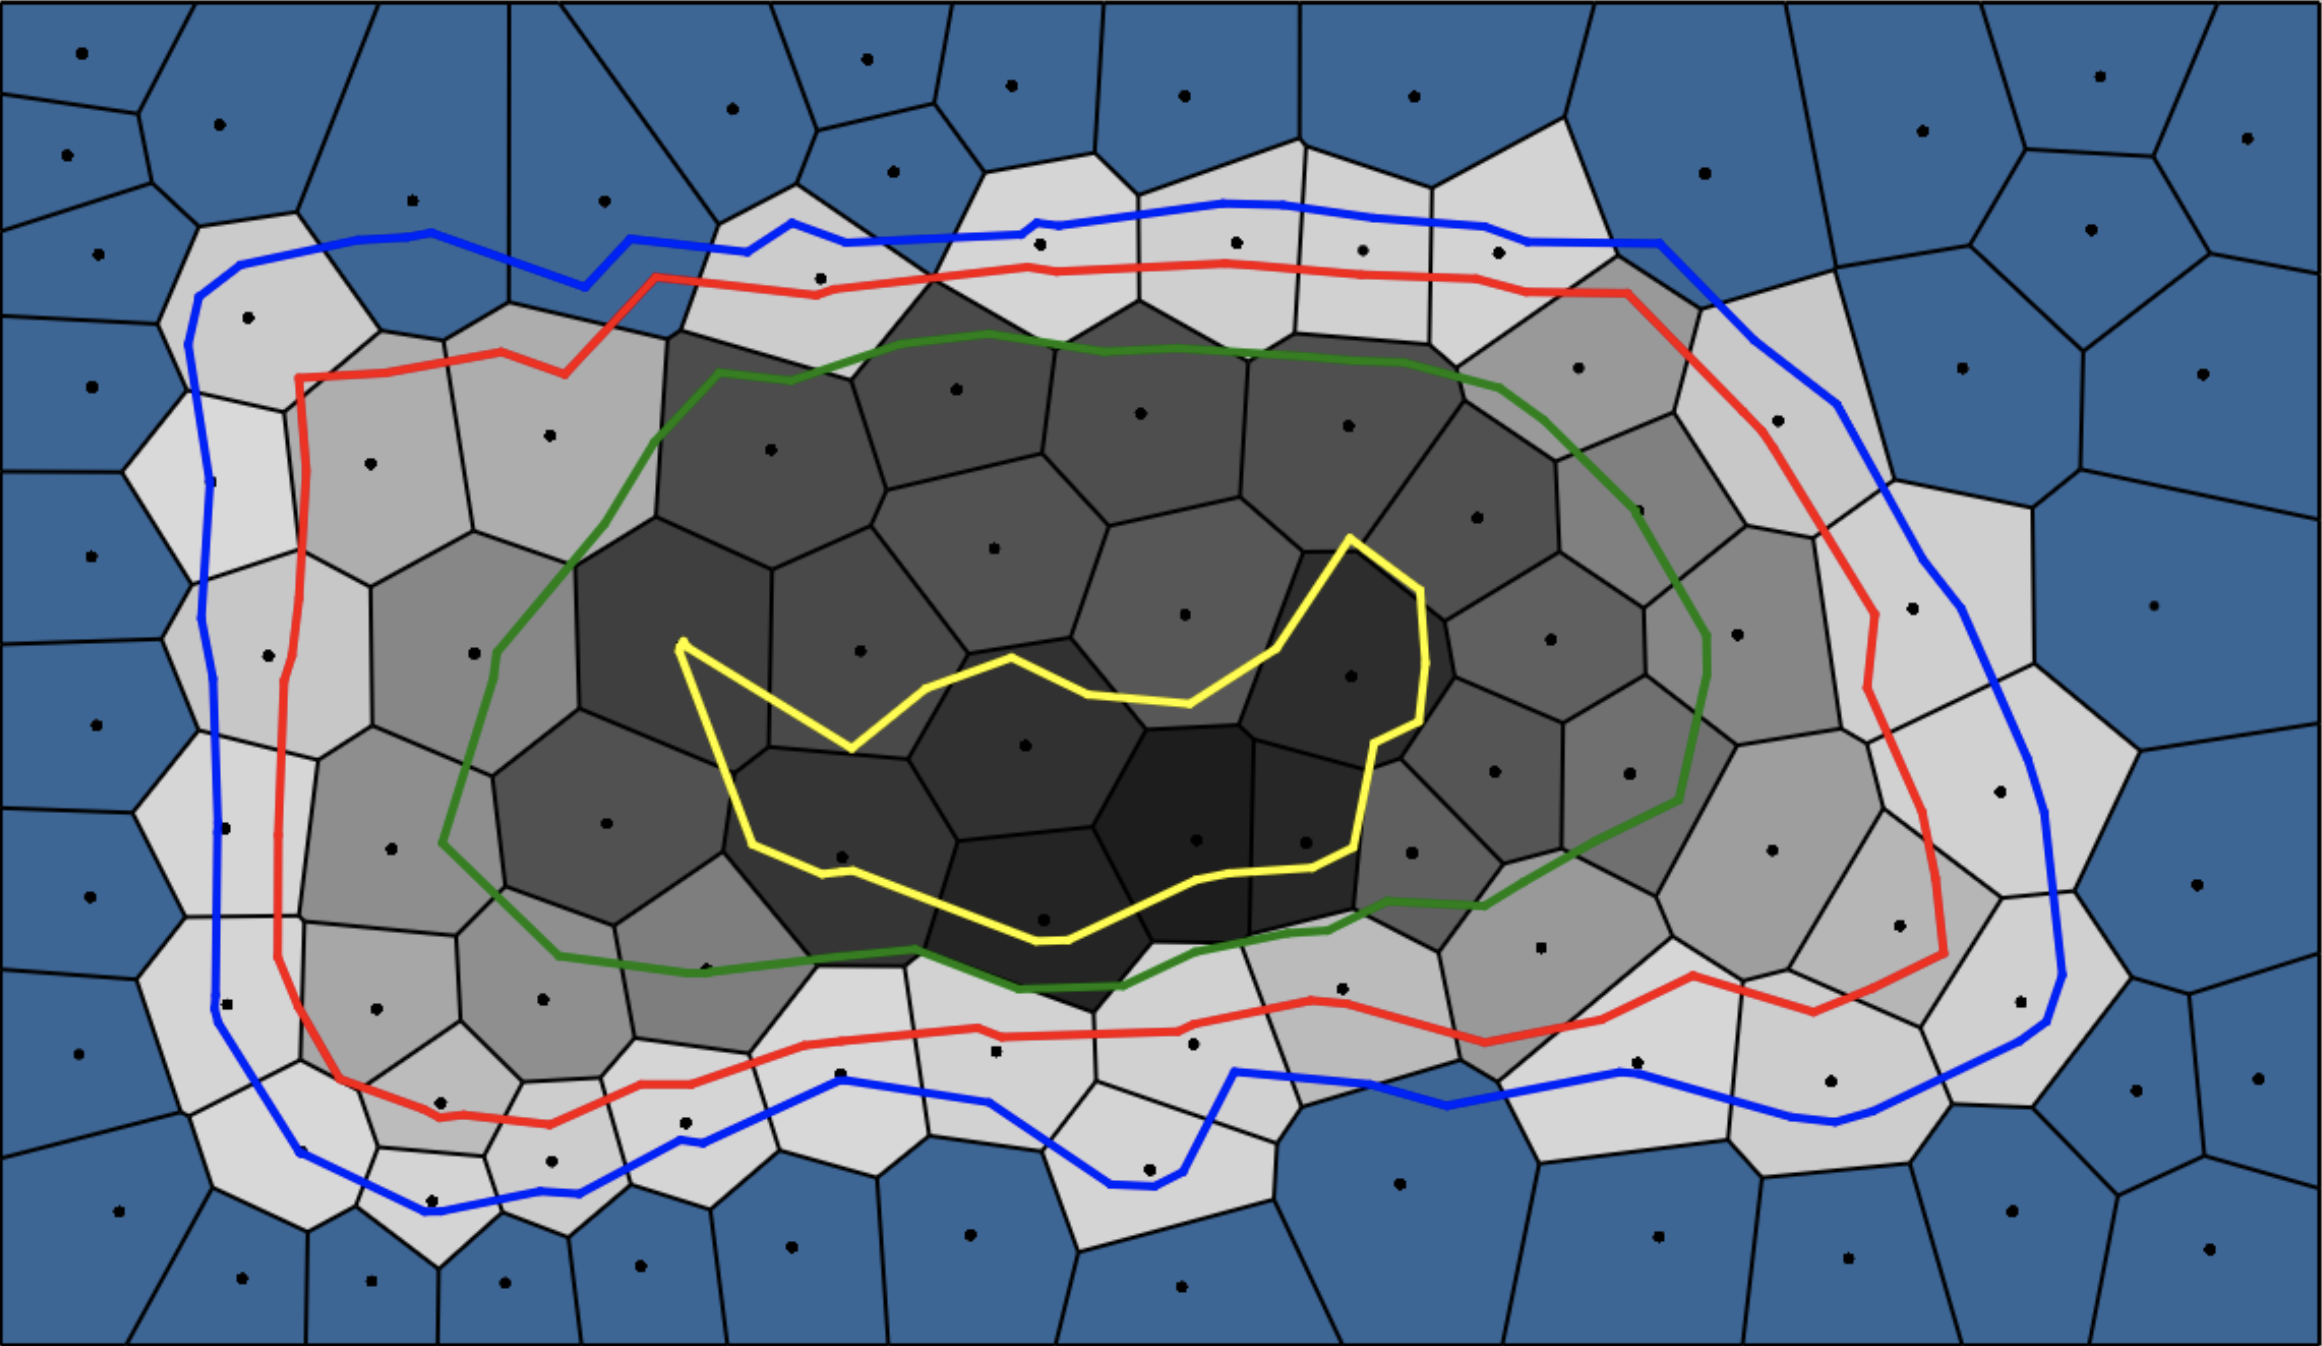
\includegraphics[width=\textwidth]{section04/assets/Map-contourline.png}
  \caption{A map with contour lines}
  \label{fig:contour line}
\end{figure}

\subsubsection{Warp Tool}
As mentioned in the previous section, the user needs to edit the map manually. So we provided several interactive methods, the most important of which is the warp tool. The warp tool is rendered as a circle that follows the mouse movement, and its role is to change the specific attribute values of all sites in the range.

In terms of elevation, we assigned a property called ``delta'' for each site object, which is the factor that determines the elevation. The user can click and drag the warp tool to change the elevation of the selected sites accordingly. In general, the longer the distance is dragged, The more values are changed. The value of elevation is the product of the delta and the increment value manually set by the user. Within the radius of the warp tool, the elevation value of sites in the center position changes more than the edge position.

The user first selects one of the two modes of ``increase'' or ``decrease.'' Correspondingly, the attribute value of the site is increased or decreased under the operation of the warp tool. Also, the size of the warp tool can be enlarged or reduced by the mouse wheel.

\subsubsection{Layers}
In our design, 5 different layers were applied to the map. Each layer comes with two modes, ``view'' and ``edit.'' Once the user has checked the edit option of a layer, its view option would also be checked; once the view option of a layer is unchecked, its edit option would also be unchecked. We always keep at least one layer viewable to ensure the normal display of the map if the user unchecks all of them. The user can view them by checking different layers, and layers can be superimposed on each other. For each polygon, we took the average of the sum of the currently selected layers of color values as its background color.

Just like introducing the concept of elevation and assigning it to sites, we then assigned ``affluence'', ``desirability'', ``district'', ``buildings'' as attributes to each site.

\subsubsection{City Wall}
The basic idea is to assign the ``wall'' attribute to each site and then give it an initial value with 0, which means there are no walls in this district. Another value is 1, representing there is the city wall in this district. The user increases or decreases the value of the wall by using the warp tool to render or erase the city wall. We used the d3.topojson library to merge all the districts with walls, which returned multiple merged polygons. Interior borders shared by adjacent polygons in merged polygons are removed, as we can see in Figure \ref{fig:city wall and classification}.

\begin{figure}[htbp]
  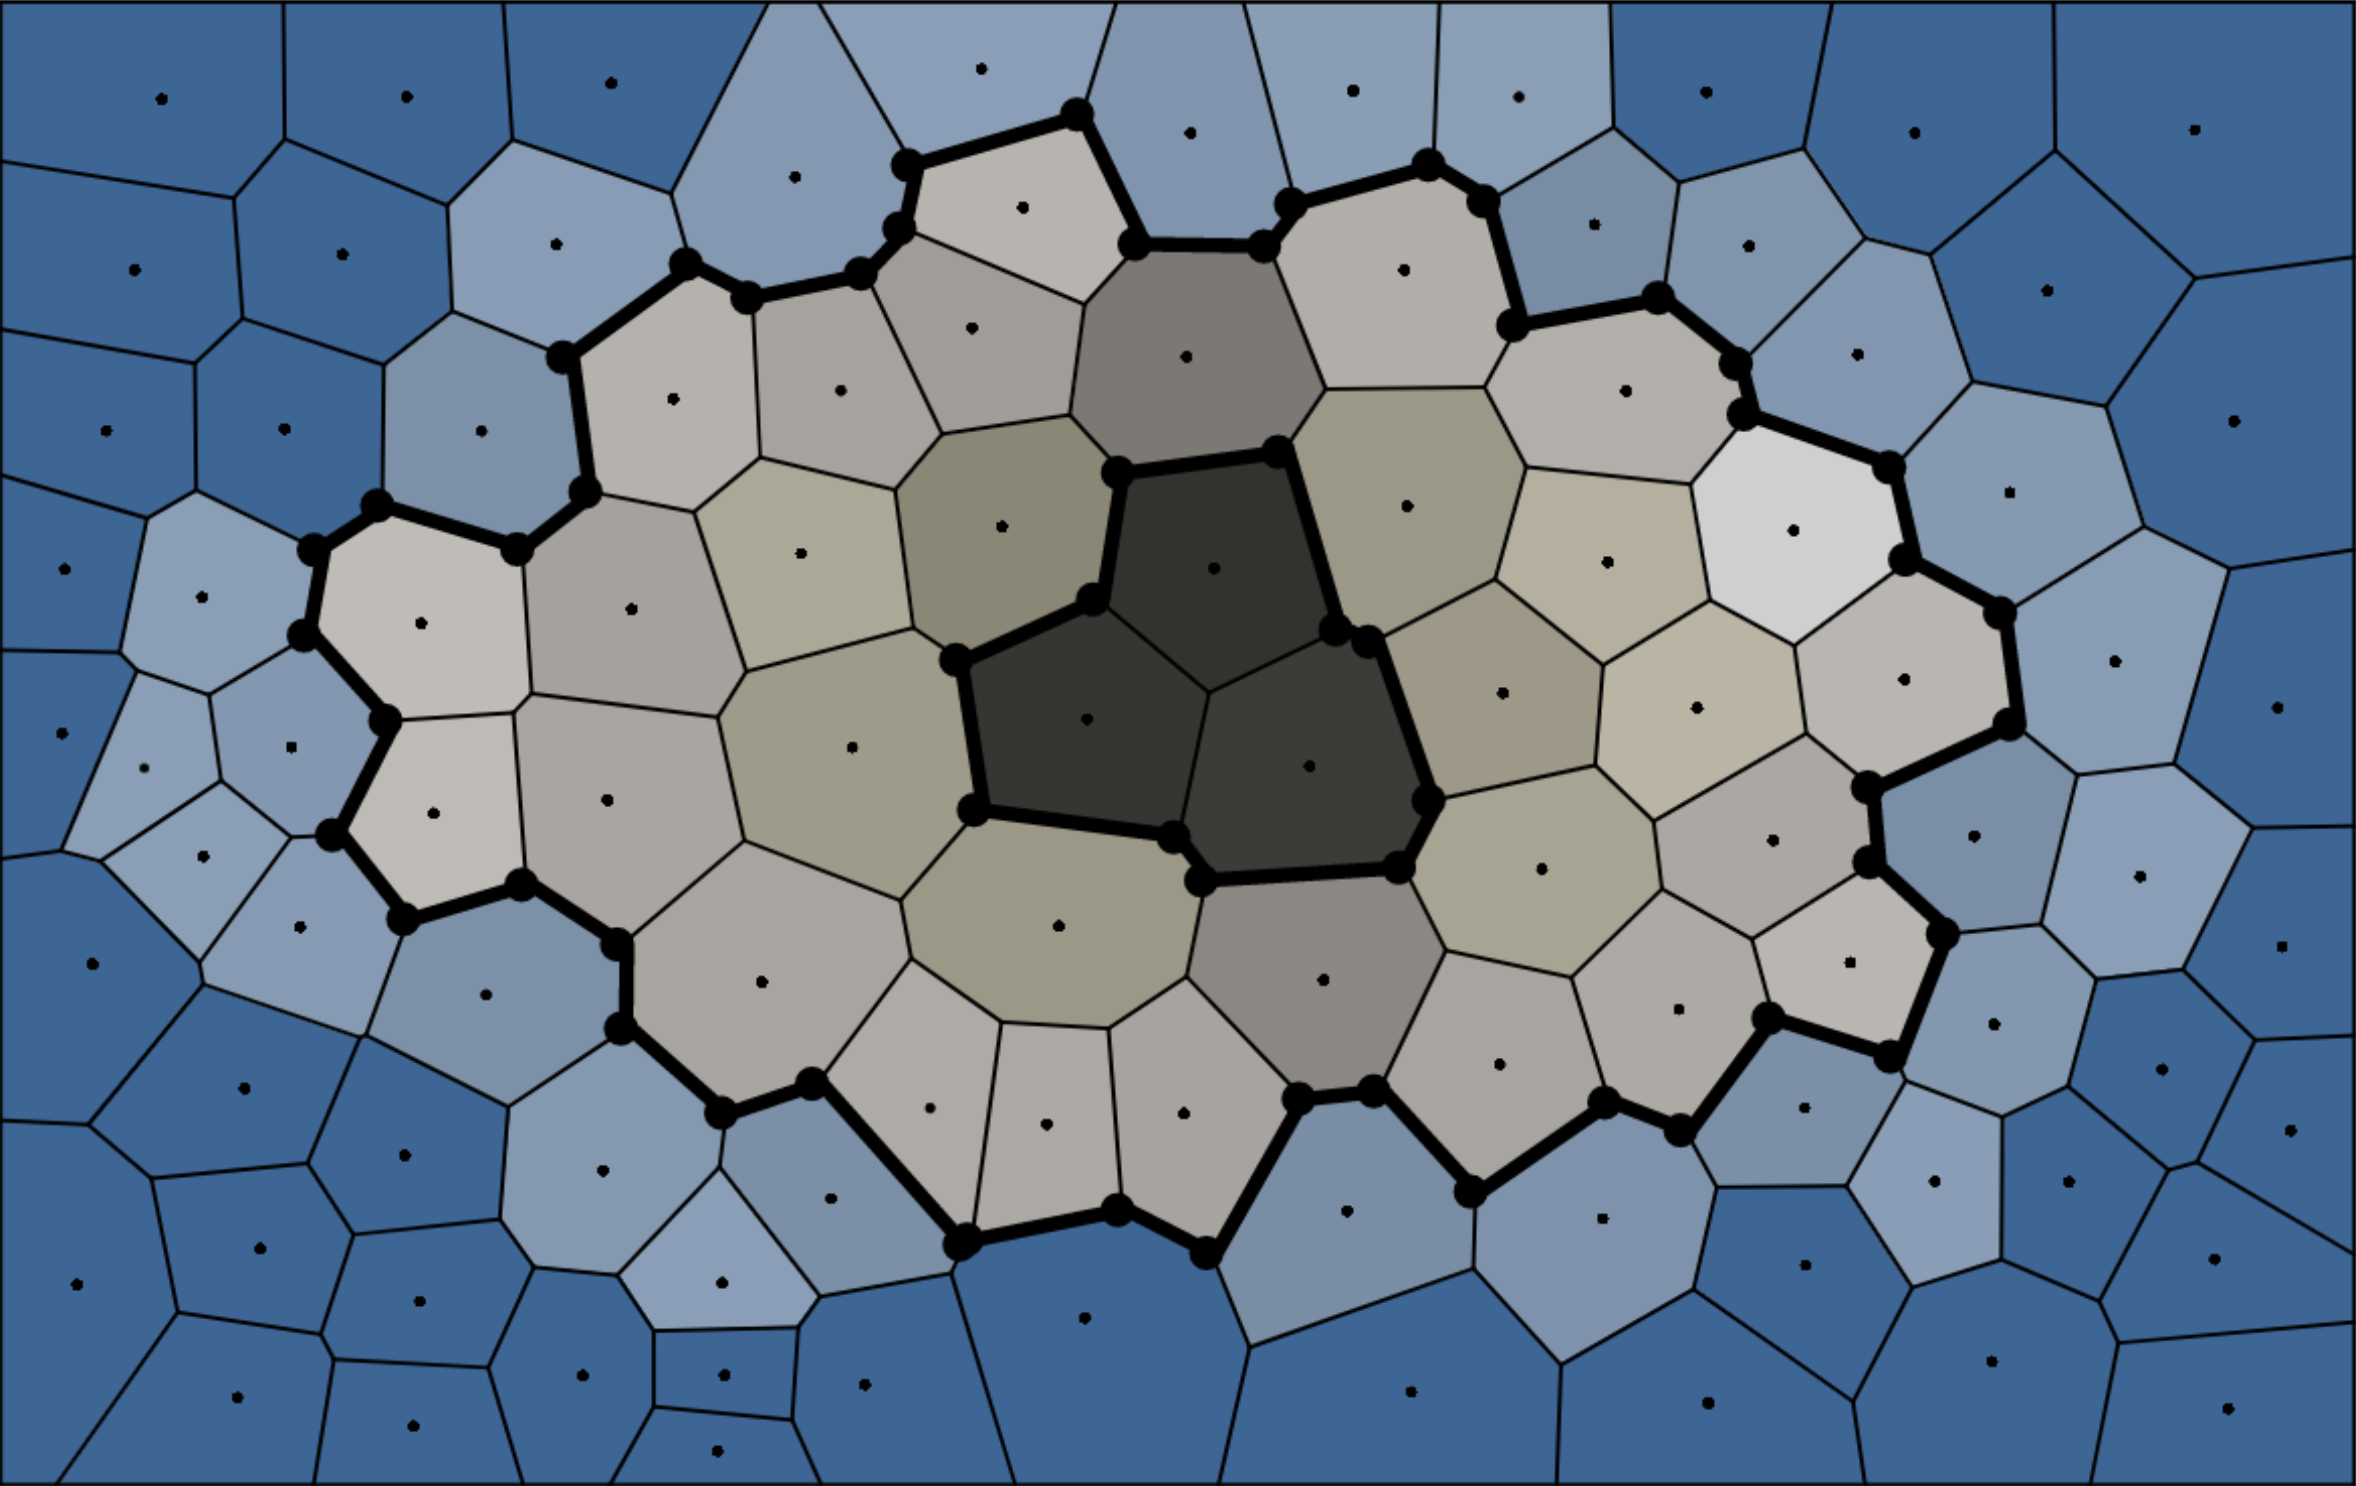
\includegraphics[width=\textwidth]{section04/assets/Map-wall.png}
  \caption{A map with walls and classification}
  \label{fig:city wall and classification}
\end{figure}

\subsubsection{Types}
As we mentioned in the design phase, the city map was subdivided into 13 types, and we assumed that the value of desirability determines most of them. The equation and the assignment conditions are listed below:

\[ desirability = (elevation + affluence) / 2 \]

\begin{enumerate}
  \item castle: $\mathbf{max}\,desirability$
  \item empty: $desirability = 0 \, \wedge \, (waterline < desirability \leq 0.45)$
  \item farm: $waterline < desirability \wedge elevation <= 0.45$
  \item harbor: $\{poor, water\} \subset \{neighbours\}$
  \item medium: $0.6 < desirability > 0.8$
  \item military: The military always surrounds the castle
  \item park: $\{poor, medium, rich\} \subset \{neighbours\}$
  \item plaza: $\{poor, medium, rich\} \subset \{neighbours\}$
  \item poor: $waterline < desirability \geq 0.6$
  \item religious: $Math.random() > 0.99 \, \wedge \, \mathbf{count} \{religious\} < 2.5 / 100 * \mathbf{count} \{polygons\}$
  \item rich: $0.8 \leq desirability \geq 1$
  \item university: $\{rich, rich, rich, rich\} \subset \{neighbours\} \, \wedge \, \mathbf{count} \{university\} < 2.5 / 100 * \mathbf{count} \{polygons\}$
  \item water: $elevation \leq waterline$
\end{enumerate}

In our design, sites closest to the boundary can only be assigned as empty, farm, or water. Different types of districts are represented by different background colors.

\subsubsection{Blocks}
One of the most important parts is the generation of buildings, which is procedural. Before generating the buildings, we first introduced the concept of a block. A district may have many blocks, and a block may contain many buildings.

The main idea of creating buildings is polygon splitting. We used a third-party library called poly-split-js.js written by Kladess \cite{web:Poly-split-js}, that implemented a polygon-splitting algorithm written by Sumit Khetarpal \cite{web:Polygon-splitting}. The algorithm splits polygons into any number of equal areas while ensuring the minimum length of line based cuts. It also works for both convex and concave polygons, as long as they do not have non-manifold vertices, and can be traversed with a single loop. In a nutshell, this algorithm is designed to divide a polygon into two by their area ratio. It receives two parameters: the vertex set of the polygon to be split and the area ratio of the polygons to be input. It returns the vertices sets Polygon1 and Polygon2 of the two split polygons, and a secant line called Cutline.

We split all polygons (except water, park, and castle) into blocks, to obtain the preliminary version of the city map. Figure \ref{fig:blocks} is an example of this technique.

\begin{figure}[htbp]
  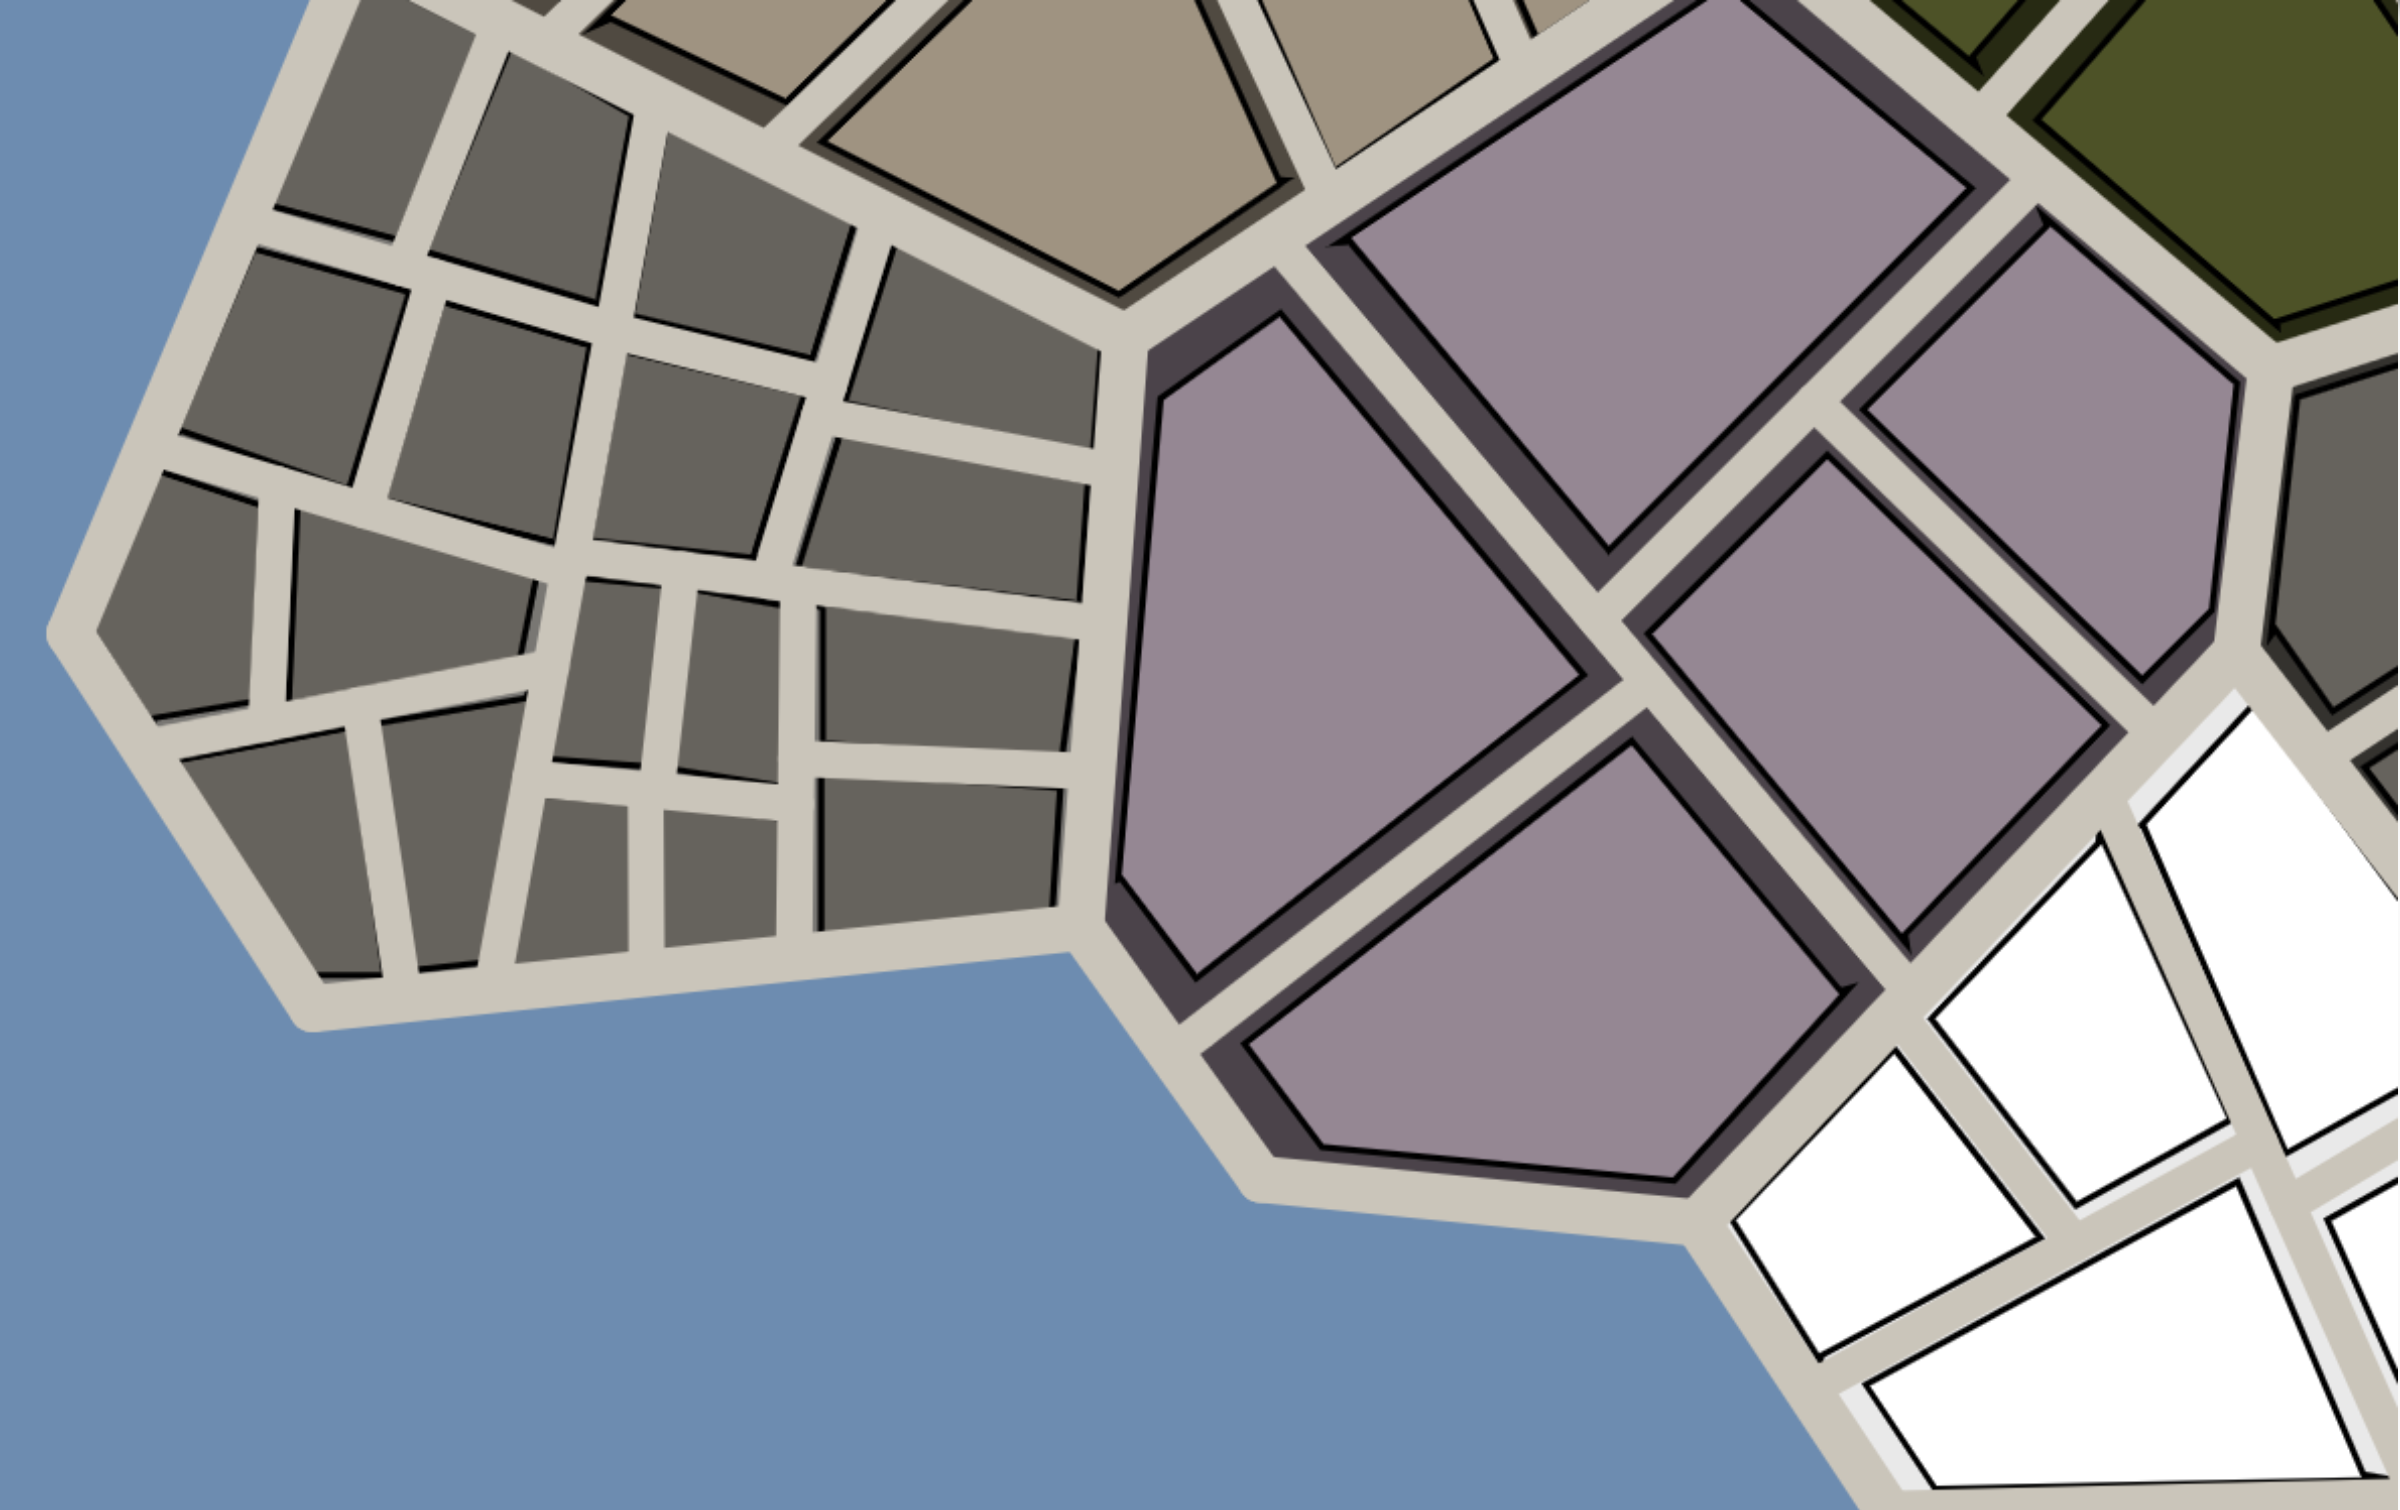
\includegraphics[width=\textwidth]{section04/assets/Map-blocks-no-buildings.png}
  \caption{A city map with each district divided into sub-blocks}
  \label{fig:blocks}
\end{figure}

\subsubsection{Streets}
A feature of this map is that of randomly generated street names. As we mentioned before, the polygon-splitting algorithm returns two polygons and a cut line. This cut line is the key to our implementation of the streets. Because there are no streets between the buildings, we only considered the streets in the blocks and the streets between districts.

First, each edge of each district is a street, and each edge of each block is also a street. Each cut line participating in the split block is also a street.

Considering that each polygon and each of its neighbors share a common edge, we avoided repeating these edges by hashing each rendered edge. Because one edge consists of two vertices, so each edge needs to be hashed twice. Then we put these hashes into a global variable. When an edge is ready to render, we took the two hash values of this edge and compared them with all the hashed edges in the global variable. If there is the same, skip rendering it, otherwise, render and add these two hashes to the global hash collection. After rendering each edge, we cleared the hash collection in the global variable for the next rendering.

Each street has its own street name. First, we obtained a collection of random street names, and then randomly placed these street names at the midpoint of each street. Because each street is only traversed once, there would be no situation where two street names appear on one street. Then we adjusted the angle between the street name and the x-axis so that it can always be displayed well on the street. Figure \ref{fig:streets} shows the streets with street names.

As the number of polygons increases, the street would increase, and street names would inevitably repeat. We hope to solve this problem in future work.

\begin{figure}[htbp]
  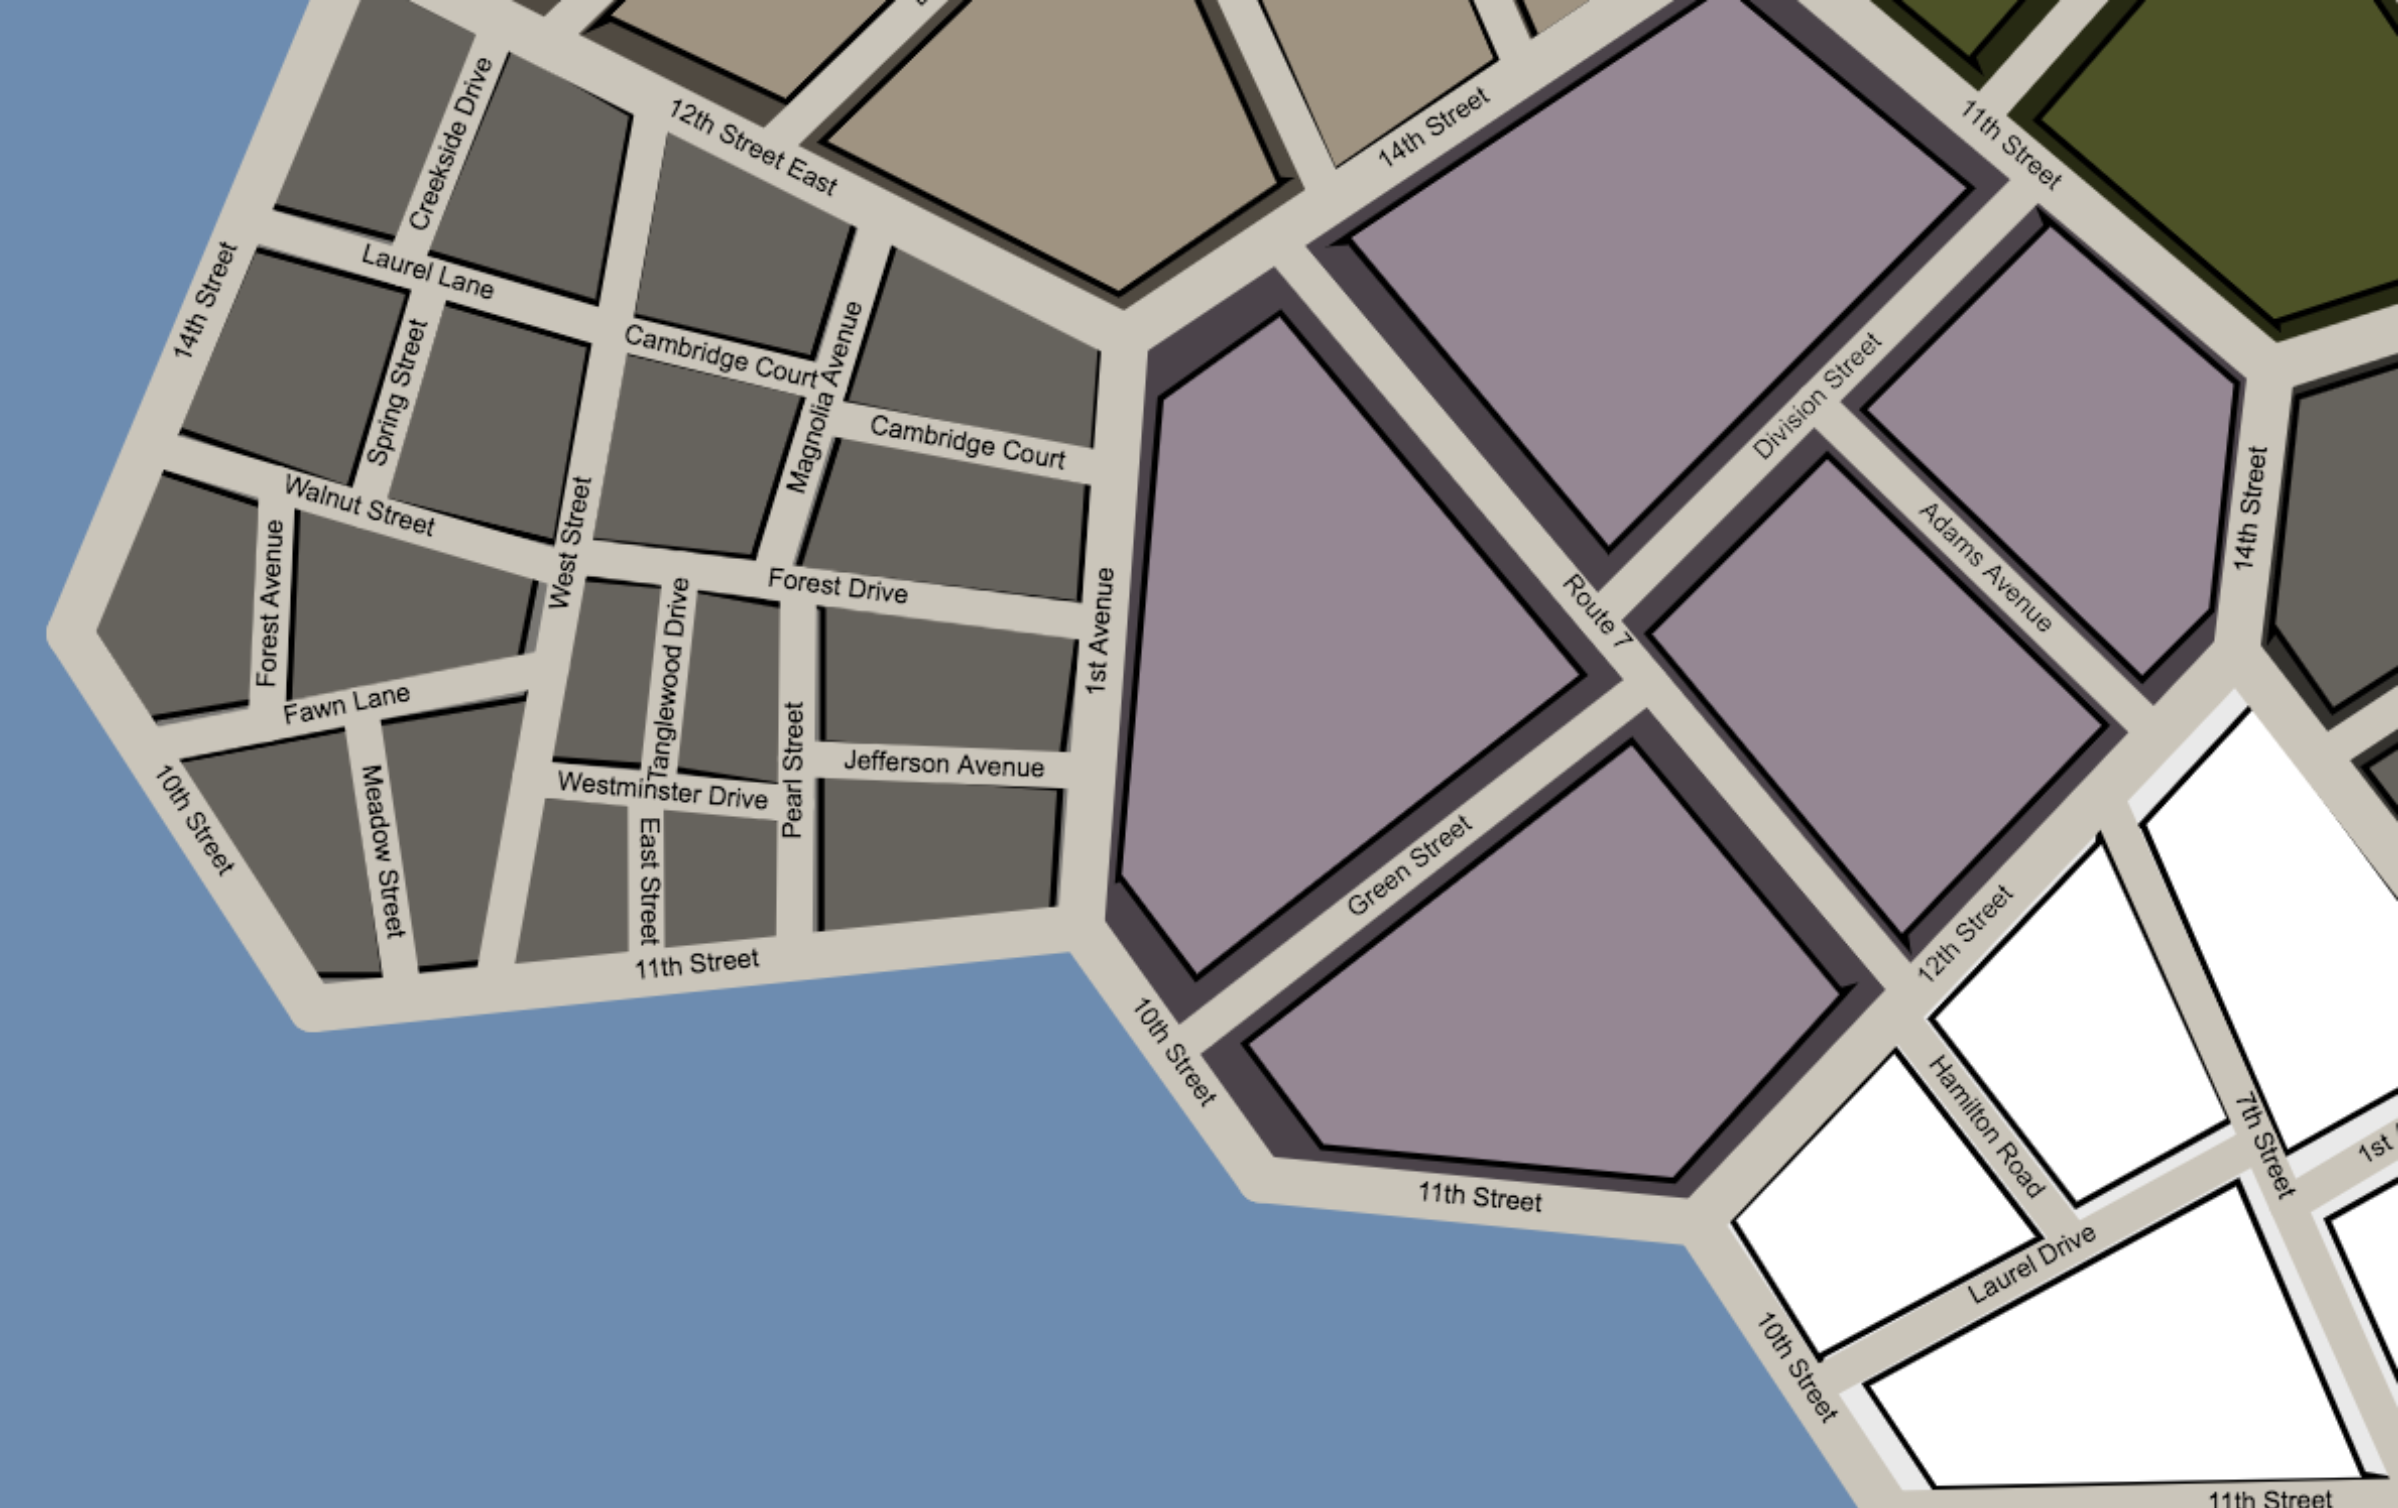
\includegraphics[width=\textwidth]{section04/assets/Map-blocks-streets.png}
  \caption{A city map with streets}
  \label{fig:streets}
\end{figure}

\subsubsection{Buildings and Details}
After getting blocks, we split them again as before. The small polygons returned this time are treated as buildings, which are located in blocks. We have previously defined several types of districts, some of which do not need to be split, for example: water, castle, and park. Some of them require unique segmentation methods, such as the farm.

For farms, it only needs to be split 2 or 3 times, unlike other ones that have been split a dozen times. These split larger polygons are pieces of the farm, we randomly made some diagonal lines to be treated as fields, and then changed the background color to the wheat color that echoes the farm. With the field, of course, the farmer’s house is indispensable. When we divide the buildings, we only need to keep a small polygon as a house. And not every farm needs a house, so we reduce the probability of splitting farms, let it occasionally do a building-level segmentation.

Besides, for the type harbor, we got the inspiration from the Medieval Fantasy City Generator and introduced the concept of deck, which is randomly generated and of moderate length. Figure \ref{fig:buildings} is the implementation of buildings and details.

Since the map would be filled with polygons in an instant, we designed such a mechanism, and the precondition is the map can be zoomed in or out normally: when the map is zoomed in to a certain extent, these buildings would be displayed. For example, when the map is enlarged to 2 times, the street names will be automatically displayed, when it is enlarged to 3 times, all the buildings will be rendered. On the one hand, the map looks much better, and on the other hand, the rendering work of the browser has been lightened, and the performance of the generator is improved.


\begin{figure}[htbp]
  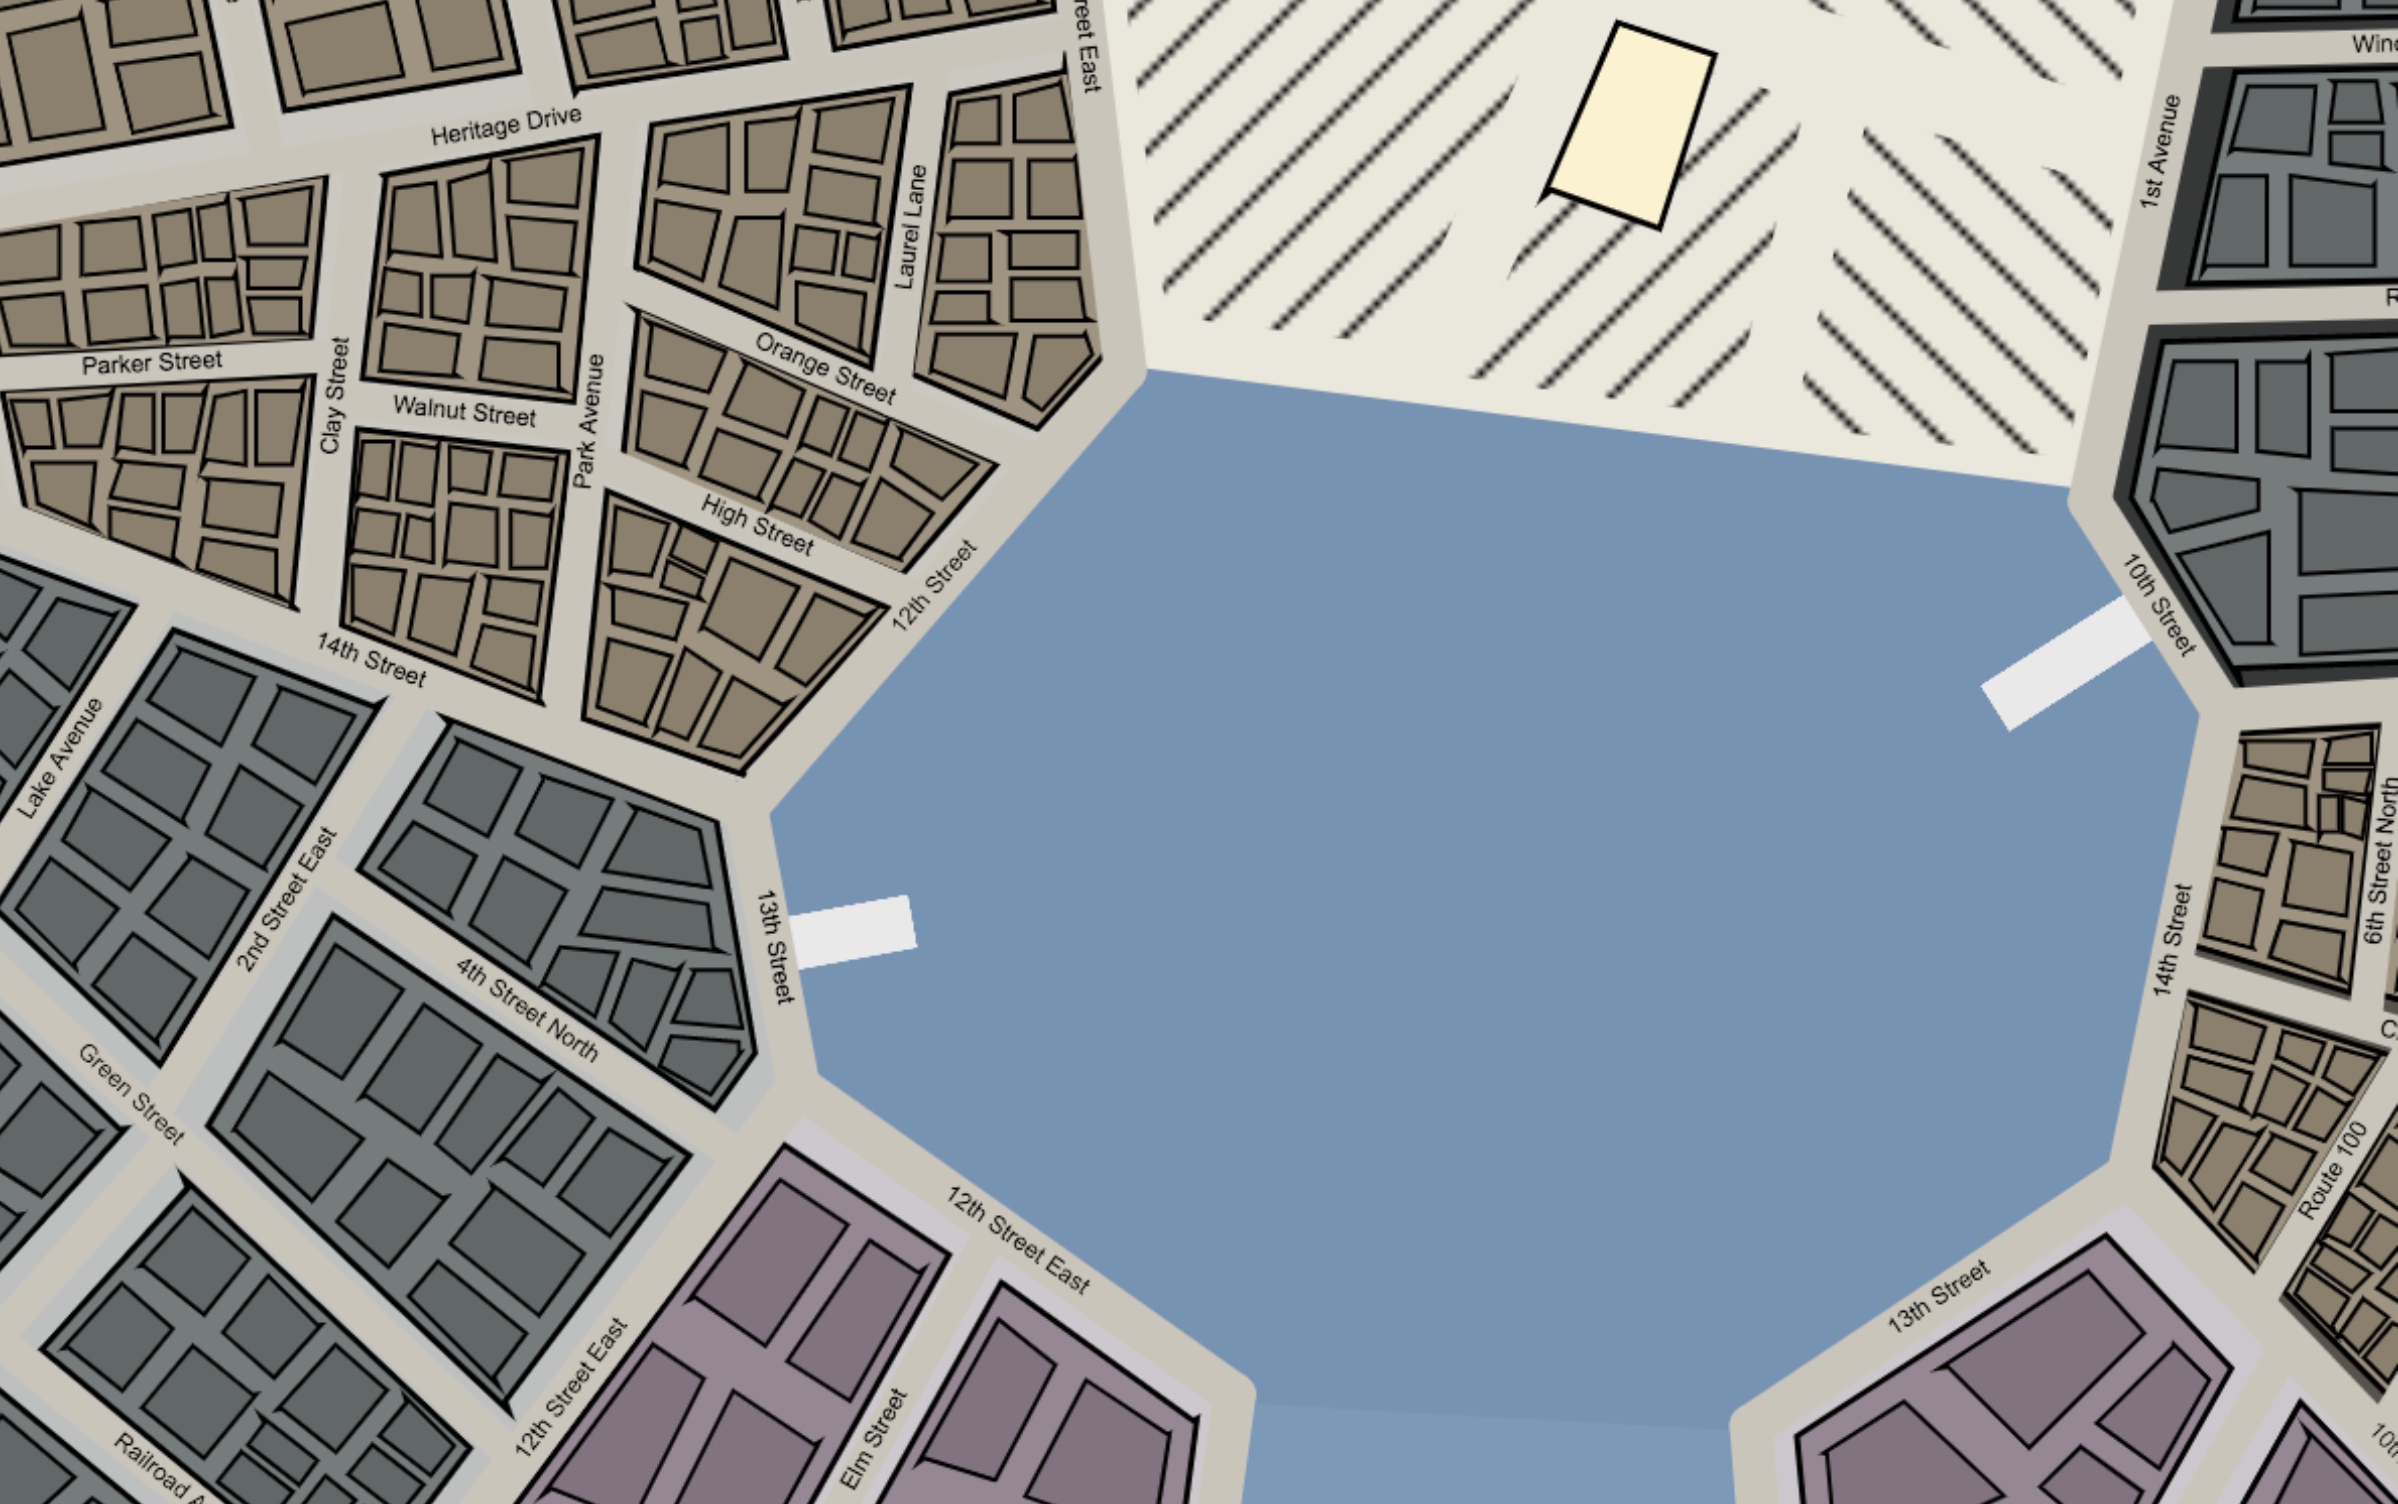
\includegraphics[width=\textwidth]{section04/assets/Map-details.png}
  \caption{A city map with buildings and details}
  \label{fig:buildings}
\end{figure}

\subsubsection{Graph Data Structure}
Figure \ref{fig:Code graph} is the core code that generates the graph and shows the graph data structure. ``this.sites'' creates random sites (points) within the scope of the Voronoi diagram (Canvas). In case of sites being too close to the boundaries, we set a padding value for boundaries. ``this.voronoi'' creates a new Voronoi layout with default x and y accessors and a null extent. ``this.diagram'' returned by Voronoi diagram object has the following properties: edges, links, cells and triangles, which respectively represent the set of edges of polygons, the set of links based on sites, the set of vertices of polygons, and Delaunay triangulation of the specified data array as an array of triangles.

The ``relaxAndReassignSites()'' method relaxes sites using Lloyd's algorithm and assigns the attributes we need to each site. The ``makeEdge()'' method accepts one parameter: the diagram object, and then simply converts the properties of the Edge object to the format we need. The ``makePolygons()'' accepts two parameters: the sites object and the diagram object, it converts the cells object from the diagram object into the format we need, assigns the properties we need to each cell, and returns new polygon objects.

\begin{figure}[htbp]
  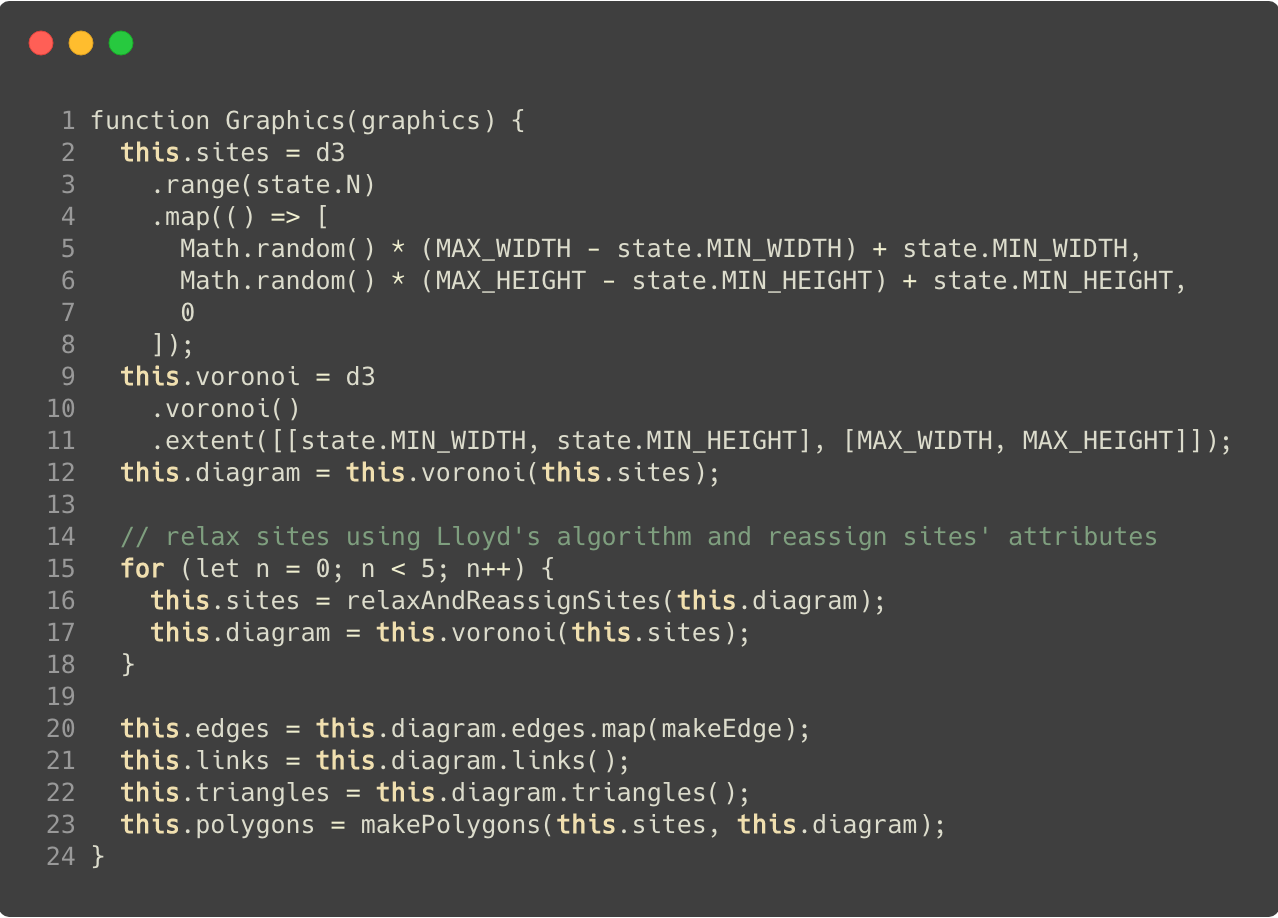
\includegraphics[width=\textwidth]{section04/assets/Graphics.png}
  \caption{Core code that generates the graph and shows the graph data structure}
  \label{fig:Code graph}
\end{figure}
